%%%%%%%%%%%%%%%%%%%%%%%%%%%%%%%%%%%%%%%%%%%%%%%%%%%%%%%%%%%%%%%%%%%%%%%%%%%%%%%%%
% MICAI / Springer LNCS submission
% "Feasibility-Preserving Multi-Objective Harris Hawks Optimization
%  for Employment-Based Visa Allocation"
%
% Compile: pdflatex main  (x2-3 passes to resolve refs)
% Bibliography: inline thebibliography (no BibTeX pass needed).
%
% ---------------------------------------------------------------------------
% DOUBLE-BLIND SUBMISSION:  MICAI reviews anonymously. To anonymize, (1) comment
% out the \author / \institute blocks below and use the ANONYMOUS block marked
% "% >>> REVIEW", (2) comment out the Acknowledgements, and (3) remove the repo
% URL in the Data Availability statement. The body is otherwise identical.
%%%%%%%%%%%%%%%%%%%%%%%%%%%%%%%%%%%%%%%%%%%%%%%%%%%%%%%%%%%%%%%%%%%%%%%%%%%%%%%%%
\documentclass[runningheads]{llncs}

% --- A4 trap fix: force a true A4 MediaBox without touching the LNCS text block.
\AtBeginDocument{\pdfpagewidth=210mm \pdfpageheight=297mm}

\usepackage[T1]{fontenc}
\usepackage[utf8]{inputenc}
\usepackage{lmodern}   % scalable fonts (required for microtype expansion)
\usepackage{graphicx}
\usepackage{xcolor}
% amsmath + llncs emit one benign "Unable to redefine math accent \vec" warning
% (modern robust accents); silence just that during amsmath's load, then restore.
\makeatletter
\let\vp@oldwarn\PackageWarningNoLine
\renewcommand\PackageWarningNoLine[2]{}
\usepackage{amsmath,amssymb}
\let\PackageWarningNoLine\vp@oldwarn
\makeatother
\setlength{\emergencystretch}{1em}  % gentle: absorb tight lines in narrow columns
\usepackage{booktabs}
\usepackage{array}
\usepackage{float}
\usepackage{algpseudocode}
% lightweight "algorithm" float (avoids the algorithms bundle; on Overleaf the
% standard \usepackage{algorithm} also works and yields the same result)
\floatstyle{ruled}
\newfloat{algorithm}{tbp}{loa}
\floatname{algorithm}{Algorithm}
\usepackage{microtype}
\usepackage[hidelinks]{hyperref}
\usepackage{url}
\renewcommand\UrlFont{\color{black}\rmfamily}

% consistent metric/acronym capitalization
\newcommand{\HV}{\textsf{HV}}
\newcommand{\IGD}{\textsf{IGD}}

\graphicspath{{figures/}}

\begin{document}

\title{A Two-Condition Diagnostic for Decoder-Based\texorpdfstring{\\}{ }Multi-Objective Search: When Blind Sampling\texorpdfstring{\\}{ }Beats a Mismatched NSGA-II}
\titlerunning{Two-Condition Diagnostic for Decoder-Based Search}

\author{Anonymous Author(s)}
\authorrunning{Anonymous}
\institute{Affiliation withheld for double-blind review}

\maketitle

\begin{abstract}
Many hard-constrained combinatorial problems are solved by pairing a metaheuristic with a feasibility-preserving decoder, yet the true driver of performance is seldom isolated. We isolate it on a calibrated case study: allocating 140{,}000 U.S.\ employment-based visas per year under a per-country ceiling and spillover cascade---a three-objective integer program with six hard constraints. Multi-objective Harris Hawks Optimization (MOHHO) searches it through a smallest-position-value random-key mapping and a greedy assignment feasible by construction---no penalties, no repair. A controlled nine-method ladder shows why search fails. Blind random sampling beats a standard real-coded NSGA-II and a naive swarm because their realized search is \emph{degenerate}: interpolating operators barely change the decoded order, or gated acceptance freezes the population. The two corresponding conditions are necessary there, not sufficient. A BRKGA-style biased-uniform crossover that does change the order under diversity-preserving selection only ties blind sampling, and a registered eleven-level disruption sweep finds hypervolume nearly flat within that family---only the right kind of order renewal (a competent random-key swarm or permutation-native operators) reaches the top tier. We package these measurements as a cheap a priori diagnostic and stress it with registered prospective tests: the two-condition core predicted correctly; the landscape label and dose--response reading did not. Across knapsack, traveling-salesman, flow-shop, and set-covering replications, the best ladder method satisfies both conditions, while the mismatched genetic algorithm's collapse below blind sampling is landscape- and configuration-specific. A Taguchi design fixes the shared parameters; the recovered front Pareto-dominates the first-in, first-out incumbent and yields an auditable trade-off menu.

\keywords{Multi-objective optimization \and Harris Hawks Optimization \and Constraint handling \and Random-key decoder \and Permutation encoding \and Taguchi design of experiments \and Resource allocation}
\end{abstract}

%===============================================================================
\section{Introduction}
\label{sec:intro}

Each fiscal year the United States Congress authorizes approximately 140{,}000 employment-based (EB) immigrant visas, distributed across five categories (EB-1 to EB-5). Two structural rules govern the distribution: a \emph{per-country ceiling} ($P_c \approx 25{,}620$ visas, the statutory 7\,\% cross-preference limit over the combined family-sponsored and employment-based preference totals~\cite{uscis}) that no single country may exceed, and a \emph{spillover} mechanism that cascades unused visas across categories (EB-4/5 $\rightarrow$ EB-1 $\rightarrow$ EB-2 $\rightarrow$ EB-3). The incumbent system processes petitions strictly first-in, first-out (FIFO) by priority date. In our calibrated instance, the interaction of these rules creates measurable inefficiencies: two countries concentrate roughly three-quarters of demand and accumulate waits of 10--13 years, while the clash between per-country and per-category ceilings leaves thousands of visas unused.

This matters beyond accounting. Behind every backlogged petition is a household whose relocation, employment, and family reunification hinge on a priority date, so the allocation rule has direct welfare consequences. The problem admits three legitimate, mutually conflicting goals: serve the longest-waiting petitions (\emph{efficiency}), distribute opportunity evenly across nationalities (\emph{equity}), and waste no visas (\emph{utilization}). No single allocation optimizes all three; the policy-relevant object is the set of best compromises---a Pareto front. Algorithmic assignment of people to scarce slots has been studied most prominently for refugee resettlement~\cite{bansak}; our contribution is methodological---how to search such constrained allocation spaces reliably---rather than a new matching-market design.

Computing that front is hard for three reasons. First, the allocation is \emph{combinatorial}: it assigns integer visa counts to 105 country$\times$category groups under six simultaneous constraints, and its feasible set generalizes the multidimensional knapsack problem, which is NP-hard~\cite{garey}. Second, the objectives are genuinely conflicting, so the solution is a front rather than a point. Third---and most often underestimated---the \emph{hard constraints} are unforgiving: a continuous population metaheuristic naturally proposes infeasible candidates, and the usual remedies (penalty functions, aggressive repair) either require delicate tuning or distort the very search landscape the metaheuristic explores.

We address these challenges with a multi-objective adaptation of Harris Hawks Optimization (MOHHO) whose centerpiece is a \emph{feasibility-preserving decoder}. Our central contribution is methodological: a controlled, mechanistically explained account---developed on the visa problem and stress-tested across four structurally distinct multi-objective problems---of when decoder-based search beats blind sampling, distilled into a two-condition diagnostic that a practitioner can run before committing a full experimental budget. Concretely, this paper makes five contributions. \emph{(i)}~A decoder that couples a smallest-position-value (SPV) random-key mapping with a deterministic greedy assignment, guaranteeing all six policy constraints \emph{by construction}---without penalties or repair, and therefore without perturbing the search landscape. \emph{(ii)}~A calibrated, constraint-heavy allocation case study on which a multi-objective Harris Hawks optimizer with a crowding-pruned external archive recovers a Pareto front of policy trade-offs that dominates the FIFO incumbent. \emph{(iii)}~A Taguchi L9 design that fixes the population size and iteration budget shared by every ladder method, so that cross-method comparisons are not confounded by per-method tuning. \emph{(iv)}~A controlled nine-method ladder (including a representation-matched \emph{Discrete-MOHHO} used as the swarm-side mechanism check), a $2\times2$ isolation experiment, and a direct operator-order-preservation measurement (Kendall $\tau$ through the decoder); together these yield the two-condition diagnostic---operators must change the decoded order and selection must preserve diversity---validated predictively on a BRKGA-style crossover not used to formulate it, which sharpens the two conditions from a binary rule to a necessary-but-graded one. \emph{(v)}~A reproducible empirical protocol (30 seeds, omnibus Friedman/Nemenyi tests with effect sizes, domination of FIFO, robustness across five perturbed-demand instances) with a four-structure generalization---knapsack, traveling salesman (TSP), and flow-shop---and a registered prospective test on a fifth, unseen problem (set covering), separating the transferable regularity (a method satisfying both conditions is the best optimizer on every structure, with the metaheuristic family second-order among them) from the landscape-specific drama (the collapse of a genetic algorithm (GA) below random sampling, which appears at default configuration on the budget-saturating problems and is configuration-robust only on the visa).

%===============================================================================
\section{Background and Related Work}
\label{sec:related}

\paragraph{Harris Hawks Optimization.}
Harris Hawks Optimization (HHO)~\cite{heidari} is a population-based metaheuristic inspired by the cooperative hunting of Harris's hawks. Its defining feature is a continuous transition between exploration and exploitation governed by a single physical quantity, the prey's \emph{escape energy} $E$, which decays with the iteration count; when $|E|\!\ge\!1$ the hawks explore, and when $|E|\!<\!1$ they exploit through soft or hard besieges, optionally with rapid Lévy-flight dives. HHO was introduced for single-objective continuous optimization and has since been extended to the multi-objective setting.

\paragraph{Multi-objective HHO.}
Yüzgeç and Kuşoğlu~\cite{kusoglu} adapt HHO to multiple objectives with an external archive and crowding-based leader selection, and Wang et al.~\cite{cerci} combine elite non-dominated sorting with a grid index. More recent work folds elitist non-dominated sorting into HHO directly~\cite{jangir} and enhances its operators for both single- and multi-objective settings~\cite{choo}. These variants are validated mostly on continuous benchmark functions; their application to a constrained combinatorial allocation problem, where feasibility---not just convergence---is the binding difficulty, is comparatively unexplored. Our work occupies that gap.

\paragraph{Bridging continuous search and combinatorial structure.}
The random-key representation of Bean~\cite{bean} encodes a permutation as a real vector and recovers it by sorting---the SPV rule, so named after Tasgetiren et al.~\cite{tasgetiren}. Random keys let a continuous operator move freely in $\mathbb{R}^{d}$ while a decoder interprets each point as a feasible discrete solution. We exploit exactly this separation of concerns: the hawks search a smooth box-constrained space, and a decoder absorbs all combinatorial structure. How much an operator step actually changes the decoded phenotype is the classical question of representation \emph{locality}: Rothlauf~\cite{rothlauf} formalized locality and redundancy for evolutionary encodings, and Raidl and Gottlieb~\cite{raidl} measured locality, heritability, and \emph{heuristic bias} empirically for decoder-based evolutionary algorithms (EAs) on the multidimensional knapsack; the bias half of that lens---a greedy decoder improves every candidate it touches---makes blind sampling through such a decoder a semi-greedy multistart in the GRASP (greedy randomized adaptive search procedure) sense~\cite{feo}, not a strawman (Section~\ref{sec:ablation} measures this directly). Our Kendall-$\tau$ order-preservation measurement instantiates exactly this lens for random keys under multi-objective search, and---unlike those single-method analyses---ties it causally to performance through a controlled multi-method ladder. The random-key idea itself has matured into biased random-key genetic algorithms (BRKGA)~\cite{goncalves,londe}, whose parameterized uniform crossover was designed precisely because interpolating operators move the keys without moving the decoded order, and, most recently, into a general random-key optimizer that pairs a problem-specific decoder with any metaheuristic~\cite{chaves}---the paradigm we instantiate here for HHO, and which our ladder probes directly by varying the metaheuristic while holding the decoder fixed.

\paragraph{Constraint handling in metaheuristics.}
Three families dominate (see Rahimi et al.~\cite{rahimi} for a recent survey). \emph{Penalty methods} fold constraint violations into the objective, but require problem-specific weights and blur the boundary between feasible and infeasible regions. \emph{Repair operators} project infeasible candidates back into the feasible set, but aggressive repair can collapse diversity and overwrite the stochasticity that drives exploration. \emph{Decoder (feasibility-preserving) approaches} guarantee feasibility by construction, leaving the search landscape intact. We adopt the third family: our greedy decoder makes every decoded candidate satisfy all six constraints exactly, so no penalty weight is ever tuned and no repair is ever applied.

\paragraph{Baseline and methodology.}
NSGA-II (Non-dominated Sorting Genetic Algorithm~II)~\cite{deb} is the canonical multi-objective evolutionary algorithm and our benchmark; such algorithms are the standard tooling for hard allocation and scheduling problems~\cite{zhang}. Our finding that the metaheuristic family is second-order once operators match the representation speaks directly to the metaphor-centered critique of metaheuristics~\cite{aranha,sorensen}: what our ladder rewards or punishes is measurable operator behavior, not the animal on the label. For parameter selection we use the Taguchi orthogonal-array design~\cite{montgomery}, a standard tool for tuning stochastic algorithms with few experiments and increasingly applied to metaheuristics~\cite{alrafei}. We assess fronts with the hypervolume indicator~\cite{zitzler} and with inverted generational distance and spacing~\cite{coello}, and we test significance with nonparametric procedures~\cite{derrac} and the $A_{12}$ effect size~\cite{vargha}.

%===============================================================================
\section{Problem Formulation}
\label{sec:formulation}

\paragraph{Decision variables.}
The problem is discretized into $G = C \times |\mathcal{J}| = 21 \times 5 = 105$ \emph{groups}, where each group $g$ is a (country~$c$, category~$j$) pair. The decision vector is
\(
\mathbf{x} = (x_1, x_2, \dots, x_G),\; x_g \in \mathbb{Z}^{+}_0,
\)
where $x_g$ is the number of visas assigned to group $g$. Each group has a demand (backlog) $n_g$ and a \emph{waiting weight} $w_g = t_{\text{now}} - d_g$, the years elapsed since its priority date $d_g$.

\paragraph{Problem instance.}
The demands $n_g$ and priority dates $d_g$ form a representative instance calibrated to the documented aggregate structure of the U.S.\ employment-based queue: a total backlog of about $1{,}800{,}000$ pending cases, with India ($\approx 63\,\%$) and China ($\approx 14\,\%$) together accounting for roughly three-quarters of demand, the remainder a long tail over the other countries, and decade-scale waits concentrated in the oversubscribed India and China EB-2/EB-3 categories~\cite{cato,dos}. We are explicit about provenance: the country-level totals are anchored to these published aggregates, but the per-(country, category) split and the priority dates $d_g$ are a plausible \emph{synthetic disaggregation} consistent with them, not an observed per-applicant census---only four high-demand blocs (India, China, the Philippines, and Mexico) have category-level demand grounded directly in published data, and the remainder is estimated. Section~\ref{sec:generalization} confirms the method comparison is stable under $\pm 20\,\%$ demand perturbation; we note this probes magnitude error, not structural mis-specification of the disaggregation, so the internal method comparison (identical data for all methods) is what we rely on, and the policy reading is illustrative.

\paragraph{Objectives.}
We minimize three conflicting objectives:
\begin{align}
f_1(\mathbf{x}) &= \frac{\sum_{g}(n_g - x_g)\,w_g}{\sum_{g} n_g}
&&\text{unserved waiting load (efficiency),}\\
f_2(\mathbf{x}) &= \max_{c_1,c_2 \in \mathcal{C}}\bigl|\bar{W}_{c_1} - \bar{W}_{c_2}\bigr|
&&\text{maximum inter-country disparity (equity),}\\
f_3(\mathbf{x}) &= V - \textstyle\sum_{g} x_g
&&\text{wasted (unassigned) visas (utilization),}
\end{align}
where $V$ is the total visa supply and $\bar{W}_c = \big(\sum_{g:\,c(g)=c} x_g w_g\big)\big/\big(\sum_{g:\,c(g)=c} x_g\big)$ is the visa-weighted mean wait of country $c$. Thus $f_2$ measures the gap between the longest- and shortest-waiting nationalities: the smaller $f_2$, the more equitable the distribution. By convention, a country that receives no visas takes its worst backlog wait as $\bar{W}_c$, so starving a nationality maximally penalizes equity---an unserved country is treated as maximally disadvantaged rather than silently dropped from the disparity. This makes $f_2$ an implicit anti-starvation pressure; FIFO and all reported equity solutions in fact serve every country, so the convention does not drive any headline result.

\paragraph{Constraints.}
The feasible set $\mathcal{F}$ is defined by six hard constraints:
\begin{align}
&\text{R1:}\;\; \textstyle\sum_{g} x_g \le V = 140{,}000 && \text{(total visas)}\nonumber\\
&\text{R2:}\;\; \textstyle\sum_{g:\,c(g)=c} x_g \le P_c = 25{,}620 \;\;\forall c && \text{(cross-preference country ceiling)}\nonumber\\
&\text{R3:}\;\; \textstyle\sum_{g:\,j(g)=j} x_g \le K_j^{\text{eff}} \;\;\forall j && \text{(effective per-category cap)}\nonumber\\
&\text{R4:}\;\; 0 \le x_g \le n_g \;\;\forall g && \text{(do not exceed demand)}\nonumber\\
&\text{R5:}\;\; x_g \in \mathbb{Z}^{+}_0 \;\;\forall g && \text{(integrality)}\nonumber\\
&\text{R6:}\;\; \text{FIFO order within each } (c,j) \text{ queue} && \text{(seniority within a group)}\nonumber
\end{align}
where $K_j^{\text{eff}}$ is the per-category cap after the spillover cascade. We use the statutory cross-preference country ceiling as an exogenous annual EB-side cap in this single-year model; a full legal simulation of family-sponsored interactions is outside scope. The cascade is part of the formulation for generality, but we note it is inert on the instances studied here: under the documented backlog every category is oversubscribed (demand exceeds its base cap by $3$--$22\times$), so the redistributable slack is zero and $K_j^{\text{eff}}=K_j^{\text{base}}$; spillover would bind only in an undersubscribed regime. The result is a three-objective integer program with six constraints---three binding budget caps (R1--R3), with R4--R6 honored automatically by any assignment the decoder of Section~\ref{sec:decoder} constructs---whose feasible space grows combinatorially with $G$, motivating a metaheuristic rather than exact enumeration.

\paragraph{Pareto optimality.}
We use the standard notions of Pareto dominance, optimality, and the Pareto front~\cite{coello}; MOHHO approximates the front through an external archive.

%===============================================================================
\section{Methods}
\label{sec:methods}

\subsection{Multi-objective Harris Hawks Optimization}
\label{sec:mohho}

Each hawk is a position $\mathbf{H}\in\mathbb{R}^{G}$ in the box $[0,1]^{G}$ (here $G=105$). At iteration $t$ the escape energy is
\begin{equation}
E = 2E_0\!\left(1 - \tfrac{t}{T}\right), \qquad E_0 \sim U(-1,1),
\label{eq:energy}
\end{equation}
which drives the choice among six movement operators selected by $|E|$ and uniform draws $q,r\in U(0,1)$ (Table~\ref{tab:operators}). The multi-objective adaptation introduces three elements. First, the \emph{leader} (the ``rabbit'' of the HHO metaphor) is not a single global best but a solution drawn from the external archive with probability proportional to its crowding distance, which biases search toward sparsely populated regions of the front. Second, an \emph{external archive} stores non-dominated solutions and, when it overflows, is pruned by removing the solution with the smallest crowding distance. Third, the archive is updated after every move using the non-dominance relation. A hawk's own move is accepted only if the trial dominates its current position---the canonical greedy replacement of single-objective HHO lifted to dominance; the published multi-objective variants~\cite{jangir,cerci,kusoglu} specify archives and leader selection rather than this acceptance, so the \emph{naive} configuration's failures below characterize this design choice, not those variants. The archive size is treated as a tunable parameter (Section~\ref{sec:taguchi}).

\begin{table}[t]
\centering
\caption{The six MOHHO movement operators, selected by the escape energy $|E|$ and uniform draws $q,r$. The archive's leader supplies the target (``prey'') position.}
\label{tab:operators}
\small
\begin{tabular}{cll}
\toprule
\textbf{Op.} & \textbf{Condition} & \textbf{Behavior}\\
\midrule
OP1 & $|E|\ge 1,\; q\ge 0.5$ & Exploration from a random hawk in the swarm.\\
OP2 & $|E|\ge 1,\; q< 0.5$ & Exploration relative to the population centroid.\\
OP3 & $0.5\le|E|< 1,\; r\ge 0.5$ & Soft besiege: gradual approach to the prey.\\
OP4 & $|E|< 0.5,\; r\ge 0.5$ & Hard besiege: aggressive contraction.\\
OP5 & $0.5\le|E|< 1,\; r< 0.5$ & Soft besiege with rapid Lévy dives.\\
OP6 & $|E|< 0.5,\; r< 0.5$ & Hard besiege with rapid Lévy dives.\\
\bottomrule
\end{tabular}
\end{table}

The Lévy operators OP5/OP6 issue a rapid dive; the canonical HHO evaluates two trial points there and keeps the better. To make the comparison \emph{function-evaluation fair}, we accept a single trial point per hawk per iteration, so MOHHO consumes exactly $N\times T$ evaluations---identical to NSGA-II, random restart, and the permutation-native methods, which is the common budget under which every result in Section~\ref{sec:results} is reported.

\subsection{A feasibility-preserving decoder}
\label{sec:decoder}

The HHO operators act in the continuous space $\mathbb{R}^{G}$, but the problem is combinatorial with six hard constraints. We bridge the two with the SPV rule~\cite{bean} followed by a deterministic greedy assignment (Algorithm~\ref{alg:decode}). The SPV rule turns a hawk $\mathbf{H}$ into a permutation $\boldsymbol{\pi}$ by sorting the group indices in ascending order of their key $h_g$. The greedy decoder then walks the groups in that order and fixes the model's decision variable
\begin{equation}
x_g = \min\!\bigl(n_g,\; V_{\text{rem}},\; P^{\text{rem}}_{c(g)},\; K^{\text{rem}}_{j(g)}\bigr),
\label{eq:greedy}
\end{equation}
decrementing the residual budgets of R1--R3 after each step. Because every assignment is capped by the remaining budgets and by demand, and counts are integers, every decoded vector satisfies R1--R6 by construction. No penalty term is introduced and no repair is performed, so the hawks search directly on a feasible objective landscape, preserving both the structure of HHO's cooperative foraging and its stochasticity. One property of the greedy fill should be stated plainly: it assigns each visited group its maximal feasible amount, so the decoder's image is the set of budget-\emph{saturating} feasible allocations---a strict subset of $\mathcal{F}$, not all of it. Every dominance and Pareto statement below is therefore relative to this decoder-reachable set. This is the right object here rather than a limitation: because visa waste $f_3$ is itself a minimized objective, deliberately reserving budget while applicants wait is rarely attractive; an exact bi-objective $(f_1,f_3)$ mixed-integer linear program (MILP) (Section~\ref{sec:ablation}) confirms that the few non-saturating non-dominated allocations that do exist improve no objective by a practically meaningful margin, so restricting to this subset loses nothing relevant.

\begin{algorithm}[t]
\caption{Feasibility-preserving SPV + greedy decoder}
\label{alg:decode}
\begin{algorithmic}[1]
\Require hawk $\mathbf{H}\in\mathbb{R}^{G}$; demands $n_g$; budgets $V$, $\{P_c\}$, $\{K_j^{\text{eff}}\}$
\State $\boldsymbol{\pi} \gets \textsc{ArgSortAscending}(\mathbf{H})$ \Comment{SPV: keys $\to$ permutation}
\State $V_{\text{rem}} \gets V$;\; $P^{\text{rem}}_c \gets P_c\;\forall c$;\; $K^{\text{rem}}_j \gets K_j^{\text{eff}}\;\forall j$
\For{$g \in \boldsymbol{\pi}$} \Comment{visit groups in SPV order}
  \State $x_g \gets \min\bigl(n_g,\, V_{\text{rem}},\, P^{\text{rem}}_{c(g)},\, K^{\text{rem}}_{j(g)}\bigr)$
  \State $V_{\text{rem}} \mathrel{-}= x_g$;\; $P^{\text{rem}}_{c(g)} \mathrel{-}= x_g$;\; $K^{\text{rem}}_{j(g)} \mathrel{-}= x_g$
\EndFor
\State \Return $\mathbf{x}$ \Comment{satisfies R1--R6 without repair}
\end{algorithmic}
\end{algorithm}

\begin{proposition}[Feasibility by construction]
\label{prop:feas}
For any hawk $\mathbf{H}\in\mathbb{R}^{G}$, the allocation $\mathbf{x}$ returned by Algorithm~\ref{alg:decode} satisfies all six constraints R1--R6.
\end{proposition}

\begin{proof}
The residuals are initialized to $V,\,P_c,\,K_j^{\text{eff}}\ge 0$ and, at each step, decremented by $x_g=\min(n_g,V_{\text{rem}},P^{\text{rem}}_{c(g)},K^{\text{rem}}_{j(g)})$. By induction each residual stays $\ge 0$, since $x_g$ never exceeds the current residual; hence $0\le x_g\le n_g$ (R4) and, as the minimum of nonnegative integers, $x_g\in\mathbb{Z}^{+}_0$ (R5). Because $x_g\le V_{\text{rem}}$ and $V_{\text{rem}}$ is the unconsumed total, $\sum_g x_g\le V$ (R1); likewise $x_g\le P^{\text{rem}}_{c(g)}$ and $x_g\le K^{\text{rem}}_{j(g)}$ keep the per-country and per-category sums within $P_c$ (R2) and $K_j^{\text{eff}}$ (R3). Finally, each group is a single $(c,j)$ pair sharing one priority date, so assigning the count $x_g$ serves its $x_g$ most-senior petitions, honoring FIFO order within the queue (R6). Thus $\mathbf{x}\in\mathcal{F}$ for every input, with no penalty term and no repair. \qed
\end{proof}

\subsection{Benchmarks and a representation-matched optimizer}
\label{sec:nsga}

To separate the contribution of the decoder, the representation, and the search heuristic, we compare a \emph{ladder} of methods that all share the same greedy decoder, objectives, hypervolume reference point, and $50\times500$ budget; they differ only in how they explore. Two operate on the continuous SPV random keys in $\mathbb{R}^{105}$:
\emph{(a)}~the MOHHO of Section~\ref{sec:mohho}; and
\emph{(b)}~\textbf{NSGA-II}~\cite{deb} with simulated binary crossover (SBX, $\eta_c=20$, $p_c=0.9$), polynomial mutation ($\eta_m=20$, $p_m=1/d$), binary tournament selection, and elitist $(\mu+\lambda)$ replacement.
A third, \emph{(c)}~\textbf{random restart}, draws the $25{,}000$ candidates uniformly at random (no search), isolating what the decoder alone achieves.

The ablation (Section~\ref{sec:ablation}) reveals that the continuous random-key operators are a poor match for the induced permutation landscape. We therefore also evaluate \textbf{permutation-native} methods---spanning four distinct paradigms---that act directly on permutations of the 105 groups (decoded by the same greedy procedure): \emph{(d)}~\textbf{permutation-NSGA-II} (dominance-based) with order crossover (OX) and swap mutation; \emph{(e)}~\textbf{permutation-MOEA/D} (multi-objective evolutionary algorithm based on decomposition~\cite{zhangli}), with Tchebycheff scalarization over a simplex lattice of 45 weight vectors, mating and replacement restricted to each subproblem's 10-nearest-weight neighborhood, an external archive of size 100, and the same OX${}+{}$swap operators; \emph{(f)}~\textbf{permutation-SPEA2}~\cite{spea2} (strength-Pareto, density-based environmental selection with truncation) under the same operators; and \emph{(g)}~\textbf{Discrete-MOHHO}, our representation-matched Harris Hawks optimizer. Discrete-MOHHO keeps HHO's signature---the escape energy $E$ of Eq.~(\ref{eq:energy}) scheduling exploration and exploitation, and a crowding-pruned external archive supplying the leader---but expresses every move on permutations: when $|E|\!\ge\!1$ a hawk explores by recombining (OX) with a random hawk or by a heavy random shuffle; when $|E|\!<\!1$ it besieges the leader by inheriting an order segment from it (OX) and perturbing with a number of swaps that shrinks as $|E|\to0$, with occasional Lévy-like segment reversals. Discrete HHO variants exist for single-objective settings~\cite{gezici}; we use Discrete-MOHHO not as a novelty claim but as the representation-matched swarm the mechanism check requires. Finally, prompted by the BRKGA literature~\cite{goncalves}, we add \emph{(h)}~\textbf{rk-NSGA-II (biased uniform)}: the NSGA-II skeleton of \emph{(b)} with SBX and polynomial mutation replaced by BRKGA-style parameterized uniform crossover on the keys (elite-parent gene with probability $0.7$) and per-gene random-reset mutation---a random-key method whose operators do change the decoded order, used in Section~\ref{sec:ablation} as a predictive test of the two-condition rule. All methods run for 30 independent seeds (1--30) under the identical budget.

\subsection{Evaluation protocol and indicators}
\label{sec:protocol}

We assess each approximation front with four indicators: the \emph{hypervolume} (\HV; larger is better) dominated with respect to the reference point $(10;\,16;\,20{,}000)$, an upper bound on each objective; the \emph{inverted generational distance} (\IGD; smaller is better) to a reference front $Z$ formed by the non-dominated union of the MOHHO and NSGA-II combined fronts ($|Z|=126$; because $Z$ is built from the compared methods' own fronts, we treat \IGD\ as an internal convergence/coverage indicator rather than distance to an independent ground truth, report it only for the pairwise MOHHO--NSGA-II comparison of Section~\ref{sec:vs-nsga}---never for the ladder---and rest the headline conclusions on the reference-point-robust \HV); the \emph{spacing} indicator (smaller is better) measuring uniformity; and the \emph{cardinality} of the non-dominated set. Objectives are min--max normalized before \IGD\ and spacing. Each algorithm is run for 30 independent seeds, and a \emph{combined front} is formed as the non-dominated union of its 30 per-run fronts. Because every method runs on the common seed block 1--30, paired comparisons use the Wilcoxon signed-rank test (with the Mann--Whitney $U$~\cite{derrac} as an unpaired cross-check), and effect size is the Vargha--Delaney $A_{12}$~\cite{vargha}; where one-sided $p$-values are reported the alternative direction is fixed a priori from the mechanism (decoder- and representation-matched methods are predicted to improve over the real-coded baseline), and the two-sided values lead to the same conclusions at these effect sizes. The deterministic \textbf{FIFO} baseline orders groups by ascending priority date and is decoded with the same greedy procedure, yielding $f_1=8.7891$, $f_2=13.0$ years, and $f_3=1{,}940$ wasted visas.

%===============================================================================
% >>> SECTION 5 (Taguchi) -- filled from the executed L9 experiment.
\section{Parameter Tuning by Taguchi Orthogonal Array}
\label{sec:taguchi}

Population-based metaheuristics are sensitive to their control parameters, and choosing them by trial and error is neither systematic nor reproducible. We therefore tune the two parameters that most directly govern the search effort---the population size $N$ and the iteration budget $T$---together with two secondary parameters, the external-archive size and the Lévy exponent $\beta$, using a Taguchi orthogonal-array design~\cite{montgomery}. The Taguchi method probes a four-factor space with a small, balanced set of experiments and quantifies each factor's influence through a signal-to-noise (S/N) ratio that rewards both a high mean response and low variance across replications.

\paragraph{Design.}
We use four factors at three levels each (Table~\ref{tab:l9}). The response is the hypervolume \HV\ of the final archive; because larger \HV\ is better, we use the larger-the-better S/N ratio
\begin{equation}
\mathrm{S/N} = -10\log_{10}\!\Big(\tfrac{1}{r}\textstyle\sum_{k=1}^{r} 1/y_k^{2}\Big),
\label{eq:sn}
\end{equation}
where $y_k$ is the \HV\ of replication $k$. A full-factorial design would need $3^4=81$ configurations; the L9$(3^4)$ orthogonal array estimates all four main effects with just nine. Each configuration is replicated with $r=12$ independent seeds drawn disjointly from the 30-run benchmark seeds, so the tuning data never contaminate the evaluation of Section~\ref{sec:results}.

\begin{table}[t]
\centering
\caption{L9$(3^4)$ orthogonal array, configurations, and response (12 replications per row). \HV\ is reported as mean\,$\pm$\,s.d.\ in units of $10^{6}$; S/N is the larger-the-better ratio of Eq.~(\ref{eq:sn}).}
\label{tab:l9}
\small
\begin{tabular}{ccccccc}
\toprule
\textbf{Run} & $\boldsymbol{N}$ & $\boldsymbol{T}$ & \textbf{Archive} & $\boldsymbol{\beta}$ & \textbf{\HV} $(\times 10^{6})$ & \textbf{S/N (dB)}\\
\midrule
1 & 30 & 100 & 50  & 1.3 & $0.290 \pm 0.010$ & 109.220\\
2 & 30 & 300 & 100 & 1.5 & $0.296 \pm 0.005$ & 109.419\\
3 & 30 & 500 & 150 & 1.7 & $0.292 \pm 0.010$ & 109.304\\
4 & 50 & 100 & 100 & 1.7 & $0.293 \pm 0.007$ & 109.323\\
5 & 50 & 300 & 150 & 1.3 & $0.297 \pm 0.010$ & 109.446\\
6 & 50 & 500 & 50  & 1.5 & $0.301 \pm 0.006$ & 109.560\\
7 & 70 & 100 & 150 & 1.5 & $0.301 \pm 0.008$ & 109.574\\
8 & 70 & 300 & 50  & 1.7 & $0.303 \pm 0.010$ & 109.603\\
9 & 70 & 500 & 100 & 1.3 & $0.306 \pm 0.008$ & 109.719\\
\bottomrule
\end{tabular}
\end{table}

\paragraph{Main effects.}
Averaging the S/N ratio over the levels of each factor gives the response table (Table~\ref{tab:response}) and the main-effects plot (Figure~\ref{fig:taguchi}). The ranking by S/N range is unambiguous: \emph{population size} ($\Delta=0.318$~dB) and \emph{iteration budget} ($\Delta=0.155$~dB) dominate, whereas the Lévy exponent ($\Delta=0.108$~dB) and the archive size ($\Delta=0.046$~dB) lie within the run-to-run noise. This is itself an informative result---it confirms that the two parameters flagged as needing justification are precisely the influential ones, and that the algorithm is robust to the secondary choices. The population effect is monotone and grows toward the top of the range (largest at $N=50\!\to\!70$, $+0.189$~dB), whereas the iteration effect saturates ($+0.117$~dB from $T{=}100$ to $300$, then only $+0.039$~dB to $500$), confirming that the iteration budget is past its point of diminishing returns.

\begin{table}[t]
\centering
\caption{Response table: mean S/N (dB) per factor level, range $\Delta$, and rank. Larger $\Delta$ means a more influential factor; the highest-S/N level in each row is in bold. Each $\Delta$ is computed from unrounded S/N values.}
\label{tab:response}
\small
\begin{tabular}{lccccc}
\toprule
\textbf{Factor} & \textbf{Level 1} & \textbf{Level 2} & \textbf{Level 3} & $\boldsymbol{\Delta}$ & \textbf{Rank}\\
\midrule
A: population $N$        & 109.314 & 109.443 & \textbf{109.632} & 0.318 & 1\\
B: iteration budget $T$  & 109.372 & 109.489 & \textbf{109.528} & 0.155 & 2\\
C: archive size          & 109.461 & \textbf{109.487} & 109.441 & 0.046 & 4\\
D: Lévy exponent $\beta$ & 109.462 & \textbf{109.518} & 109.410 & 0.108 & 3\\
\bottomrule
\end{tabular}
\end{table}

\begin{figure}[t]
\centering
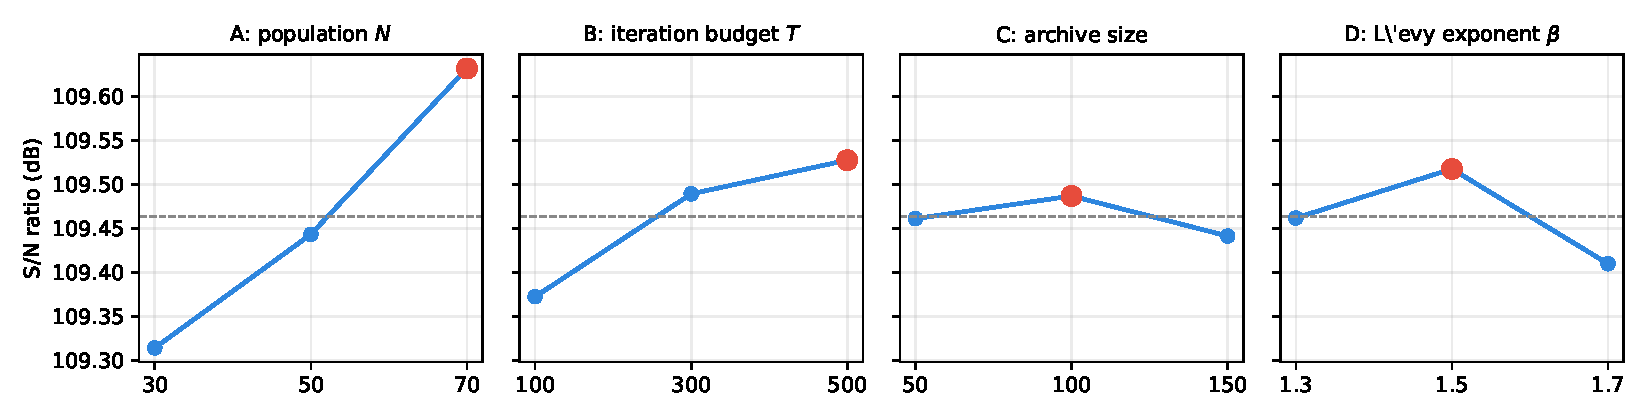
\includegraphics[width=\textwidth]{taguchi_main_effects.pdf}
\caption{Main-effects plot of the S/N ratio. The dashed line is the grand mean (109.46~dB) and the red marker the best level per factor. Population and iteration budget show clear trends (population the steeper); archive size and $\beta$ are essentially flat.}
\label{fig:taguchi}
\end{figure}

\paragraph{Optimum and confirmation.}
Selecting the best level of each factor yields the predicted optimum $N=70$, $T=500$, archive $=100$, $\beta=1.5$. Under the additive model, its predicted S/N is $\approx 109.78$~dB. A \emph{confirmation run} at that configuration (12 fresh seeds) gives an observed S/N of $109.66$~dB ($\HV = 304{,}391$). The $\approx 0.12$~dB gap between prediction and observation is small---the slight positive bias is the expected signature of an additive model that ignores factor interactions---so the additive assumption holds and the tuning is internally consistent.

\paragraph{Adopted operating point.}
The 30-run study and the NSGA-II benchmark of Section~\ref{sec:results} use $N=50$, $T=500$, archive $=100$, and $\beta=1.5$. A confirmation run at this configuration gives S/N $=109.56$~dB ($\HV = 300{,}775$), within $1.2\,\%$ hypervolume of the L9 optimum. We retain it deliberately: its \emph{sole} difference from the optimum is the population size ($50$ vs.\ $70$)---$T$, archive size, and $\beta$ all match the optimum---and increasing $N$ from 50 to 70 raises the per-iteration cost by $40\,\%$ for only a ${\approx}1.2\,\%$ \HV\ gain. Likewise $T=500$ is intentionally conservative---it exceeds by a wide margin the empirical 99\,\%-convergence point at iteration~138 (Section~\ref{sec:convergence})---so the budget cannot be blamed for any shortfall. In short, the Taguchi study turns a previously empirical choice into a justified operating point about a decibel-tenth below the L9 optimum, with the dominant factor ($T$) already at its best level.


%===============================================================================
\section{Results}
\label{sec:results}

\subsection{Combined Pareto front and domination of FIFO}
\label{sec:front}

Combining and re-filtering the 30 runs yields a front of 104 non-dominated solutions. Figure~\ref{fig:pareto3d} shows it in the full objective space and Figure~\ref{fig:pareto2d} in the $f_1$--$f_2$ projection; in both, the FIFO baseline floats above the front, visual evidence that it is dominated. The extreme solutions (Table~\ref{tab:extremes}) expose the trade-offs.

\begin{figure}[t]
\centering
\begin{minipage}[t]{0.49\textwidth}
\centering
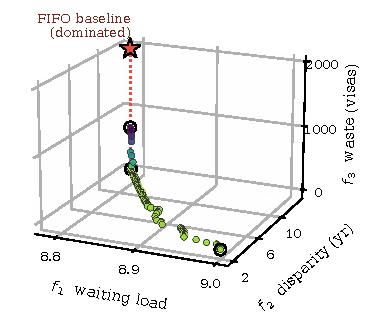
\includegraphics[width=\linewidth]{pareto3d_v2.pdf}
\caption{The 104-solution combined Pareto front over the three objectives, colored by the waste $f_3$. The FIFO baseline (red star, the isolated marker above the surface) floats above the front---the dotted drop-line marks its distance to the front's waste level---and is dominated; circles mark the extreme solutions.}
\label{fig:pareto3d}
\end{minipage}\hfill
\begin{minipage}[t]{0.49\textwidth}
\centering

\includegraphics[width=\linewidth]{pareto_f1f2.pdf}
\caption{$f_1$--$f_2$ projection of the same front, colored by $f_3$ (wasted visas). FIFO lies inside the dominated region.}
\label{fig:pareto2d}
\end{minipage}
\end{figure}

\begin{table}[t]
\centering
\caption{Extreme solutions of the combined front, compared with the FIFO baseline. The minimum-$f_1$ solution dominates FIFO (better on two objectives, equal on the already-maximal disparity).}
\label{tab:extremes}
\small
\begin{tabular}{lcccl}
\toprule
\textbf{Solution} & $\boldsymbol{f_1}$ & $\boldsymbol{f_2}$ \textbf{(yr)} & $\boldsymbol{f_3}$ \textbf{(visas)} & \textbf{Remark}\\
\midrule
Min.\ $f_1$ (least waiting) & 8.7884 & 13.0 & 680 & \textbf{Dominates FIFO}\\
Min.\ $f_2$ (most equitable) & 8.9994 & 2.0 & 0 & Radical equity\\
Min.\ $f_3$ (full use) & 8.996 & 2.46 & 0 & 100\,\% utilization\\
FIFO baseline & 8.7891 & 13.0 & 1{,}940 & Reference (dominated)\\
\bottomrule
\end{tabular}
\end{table}

The central empirical finding is that FIFO is not Pareto-optimal: the minimum-$f_1$ solution Pareto-dominates it---strictly better on waste ($f_3$ from 1{,}940 to 680 visas), tied on the already-maximal disparity ($f_2=13.0$), and negligibly better on the near-degenerate $f_1$ (8.7891 to 8.7884; the $f_1$ range is so narrow---Section~\ref{sec:discussion}---that this edge carries no practical weight). The substantive case against FIFO is therefore about waste and equity, not waiting load: 94 of the 104 front solutions reach $f_3=0$ (zero waste, which FIFO never attains), and the front spans disparities all the way from FIFO's 13.0 years down to 2.0. (The MOHHO, Discrete-MOHHO, and permutation-NSGA-II combined fronts agree within $0.3\,\%$ in hypervolume, so the policy menu does not hinge on the optimizer choice---any selected top-tier optimizer yields an essentially equivalent front.)

\subsection{Convergence and robustness}
\label{sec:convergence}

The mean hypervolume curve (Figure~\ref{fig:convergence}) reaches 95\,\% of its final value by iteration~5 and 99\,\% by iteration~135; gains beyond iteration~140 are under 1\,\%. Over the 30 runs the \HV\ distribution is narrow (mean $302{,}756$, standard deviation $7{,}138$), a coefficient of variation (CV) of 2.36\,\%, evidence of a stable and reproducible algorithm.

\begin{figure}[t]
\centering
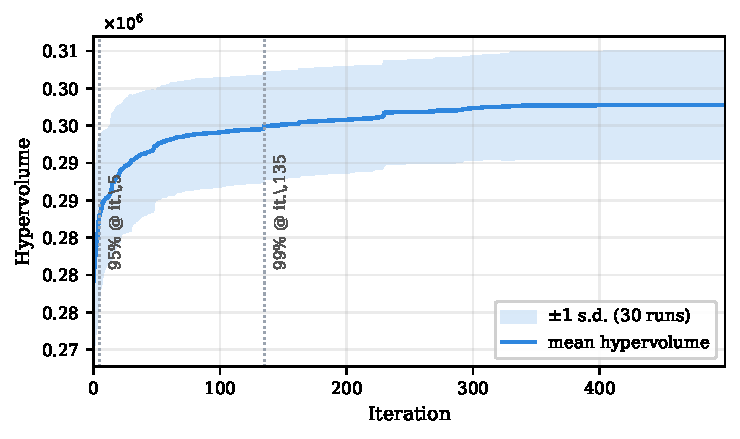
\includegraphics[width=0.72\textwidth]{convergence.pdf}
\caption{Mean hypervolume over 30 runs with a $\pm 1$ standard-deviation band. The dotted markers indicate the iterations at which 95\,\% and 99\,\% of the final \HV\ are attained; gains beyond iteration 140 are marginal.}
\label{fig:convergence}
\end{figure}

\subsection{Comparison with NSGA-II}
\label{sec:vs-nsga}

We first compare the two random-key optimizers under the identical problem, encoding, decoder, and budget of Section~\ref{sec:taguchi}. MOHHO outperforms the standard (real-coded) NSGA-II on the aggregate front-quality measures (Table~\ref{tab:nsga})---the two tie on the extreme values the decoder makes attainable for both (best $f_1$ and zero waste). MOHHO attains a higher mean hypervolume ($+3.2\,\%$) and more uniform spacing (NSGA-II edges it on $\IGD$ to the combined reference front); the hypervolume gap is significant (paired two-sided Wilcoxon on the common seeds, $p=4.4\times10^{-6}$; $A_{12}=0.85$). Figure~\ref{fig:overlay} shows the front coverage. This advantage is a property of the search dynamics, not of archiving (granting NSGA-II the identical archive barely moves it; Section~\ref{sec:ablation}): MOHHO's position updates induce genuine permutation jumps on the random keys, whereas NSGA-II's interpolating operators scarcely perturb the decoded order (Section~\ref{sec:ablation} quantifies this). That comparison, however, is only part of the story.

\begin{table}[t]
\centering
\caption{MOHHO vs.\ NSGA-II under an identical problem, encoding, decoder, and budget (30 runs each). Best value per row in bold. The FIFO point is dominated by both and is not a front.}
\label{tab:nsga}
\small
\begin{tabular}{lccc}
\toprule
\textbf{Metric} & \textbf{FIFO} & \textbf{MOHHO} & \textbf{NSGA-II}\\
\midrule
Method type & deterministic & metaheuristic & metaheuristic\\
Best $f_1$ (waiting load) & 8.7891 & \textbf{8.7884} & \textbf{8.7884}\\
Best $f_2$ (disparity, yr) & 13.0 & \textbf{2.0} & 2.25\\
Best $f_3$ (waste, visas) & 1{,}940 & \textbf{0} & \textbf{0}\\
Mean \HV\ $\pm\,\sigma$ (30 runs) & --- & $\mathbf{302{,}756 \pm 7{,}138}$ & $293{,}367 \pm 6{,}996$\\
Coefficient of variation & --- & \textbf{2.36\,\%} & 2.38\,\%\\
Combined-front \HV & --- & \textbf{320{,}984} & 316{,}060\\
Non-dominated solutions & 1 & \textbf{104} & 92\\
$\IGD$ vs.\ $Z$ (smaller better) & --- & 0.0212 & \textbf{0.0071}\\
Spacing (smaller better) & --- & \textbf{0.0106} & 0.0463\\
Significance vs.\ MOHHO & dominated & --- & $p=4.4\times10^{-6}$\\
\bottomrule
\end{tabular}
\end{table}

\begin{figure}[t]
\centering
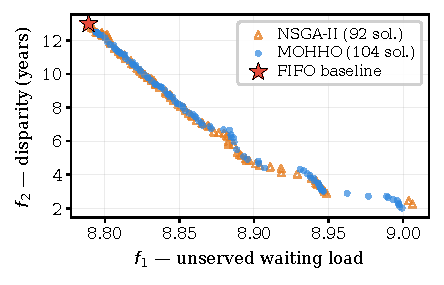
\includegraphics[width=0.62\textwidth]{nsga2_overlay.pdf}
\caption{Combined fronts of MOHHO and (real-coded) NSGA-II in the $f_1$--$f_2$ projection. MOHHO covers the front more densely and more uniformly.}
\label{fig:overlay}
\end{figure}

\subsection{Decoder, representation, and search: a controlled ladder}
\label{sec:ablation}

Section~\ref{sec:vs-nsga} compared two random-key methods. To attribute performance to its true source we now climb a ladder of methods, all sharing the decoder and a $25{,}000$ function-evaluation budget---the comparison currency (Table~\ref{tab:ladder}). The permutation-native methods inherit the Taguchi-tuned $N$ and $T$ and are not separately tuned, so any edge they show is not a tuning artifact.

\paragraph{Blind sampling beats near-identity search---but not a competent swarm.}
\emph{Random restart}---blind sampling with no search---already reaches a mean \HV\ of $310{,}214$: $5.7\,\%$ above NSGA-II and $2.5\,\%$ above the classic real-coded MOHHO (the naive swarm wins on only $10/30$ paired seeds). Under an identical function-evaluation budget the feasibility-preserving decoder shapes a landscape on which blind sampling outperforms both real-coded searches; giving NSGA-II the identical archive barely helps it ($293{,}666$ vs.\ $293{,}367$), so its deficit is not an archiving artifact. Nor is the swarm's loss an artifact of our single-trial-point budgeting (Section~\ref{sec:mohho}): the canonical two-point Lévy dive does not beat random restart either---$309{,}180$ at the matched $25{,}050$-evaluation budget ($-0.3\,\%$, paired Wilcoxon $p=0.74$), only a tie at its $42\,\%$-over-budget native schedule ($+0.1\,\%$, $p=0.45$).

Nor is blind sampling's strength mere order-level greediness: a GRASP-style semi-greedy multistart control~\cite{feo} (value-based restricted candidate list on the waiting weight, $\alpha\sim U(0,1)$ per construction, same $25{,}000$-construction budget and archive) lands $3.8\,\%$ below uniform random constructions ($298{,}531$ vs.\ $310{,}214$, $p=1.9\times10^{-9}$)---the decoder's heuristic bias~\cite{raidl} benefits every construction equally, and biasing the order toward one objective costs the diversity the front rewards. Granting the real-coded NSGA-II its own L9 design (the same nine-configuration budget as Section~\ref{sec:taguchi}; factors $N$, $\eta_c$, $p_c$, $p_m$; best configuration confirmed on the 30-seed block) does not rescue it either: the winner ($\eta_c{=}2$, $p_m{=}5/d$---mutation supplying the order disruption SBX lacks) climbs from $293{,}367$ to $308{,}082$, a statistical tie with blind sampling (two-sided $p=0.25$), still $3.2\,\%$ below the permutation tier. And a Pareto local search over swap neighborhoods (same archive and budget; a single swap is near-identity on the decoded order, so the diagnostic predicts failure here) lands $2.0\,\%$ below blind sampling ($303{,}979$, $p=3.4\times10^{-4}$). Six controls---identical archive, canonical L\'evy, GRASP, per-family tuning, local search, and the registered disruption sweep below---tell one story on this instance: nothing short of order renewal beats blind sampling. We are careful, though, not to over-read this as ``the decoder does the work'': blind sampling beats these two searches because their realized search is degenerate, not because real-coded search is hopeless. To establish this directly we built a \emph{competent} real-coded MO-HHO: HHO movement with elitist non-dominated-sorting selection and polynomial mutation replacing the dominance-gated acceptance. It is sound where the naive swarm collapses (ZDT2 hypervolume $0.99$ vs.\ $0.20$ of the true front), and at the same $25{,}000$-evaluation budget on the visa it beats random restart ($316{,}347$ vs.\ $310{,}214$; $+2.0\,\%$, paired Wilcoxon $p=5.7\times10^{-4}$, 30 seeds). A real-coded swarm can beat blind sampling; the naive one cannot. The lesson is therefore not that the decoder makes search irrelevant, but that what fails is degenerate search---near-identity operators (NSGA-II) or a frozen population (the gated swarm); see the two-condition rule below.

\paragraph{Why near-identity operators fail.}
Why does the real-coded NSGA-II fall below blind sampling? We measured the cause directly. On the SPV random keys, SBX and polynomial mutation are near-identity on the decoded permutation: over $3{,}000$ trials the Kendall rank correlation between a parent's SPV order and its child's is $\tau=0.99$. This is not an artifact of measuring on random parents or of one operator setting: measured \emph{on-trajectory}---parents drawn by the algorithm's own tournament from live populations at iterations $1$ through $499$---the correlation stays in $[0.987,0.992]$ throughout the run; and sweeping the crossover distribution index $\eta_c\in\{2,\dots,100\}$ (Figure~\ref{fig:eta}) shows that even the most disruptive crossover ($\eta_c{=}2$, $\tau{=}0.92$) leaves the real-coded GA's mean \HV\ at $305{,}293$---still below blind random restart ($310{,}214$) and far below the permutation tier. The GA perturbs the keys so little that the induced permutation barely changes, leaving it almost frozen in combinatorial space---precisely why it sinks below blind sampling, which at least draws fresh permutations. HHO's position updates, by contrast, propose large permutation jumps ($\tau\approx0$); the dominance-gated acceptance rarely admits them---only about $0.6\,\%$ of hawks move per iteration, so the realized population is largely frozen---but the external archive is fed by these rejected proposals, so the archived front still samples the decoded space far more widely than NSGA-II's near-identity proposals (hence MOHHO $>$ NSGA-II within the random-key tier). The real-coded MOHHO is thus a deliberately standard, weak baseline: on a concave benchmark front (ZDT2) its operators collapse the whole population to a corner---hypervolume around $0.20$ of the true front under every acceptance rule and every reasonable repair we tried---so our thesis rests not on the swarm being strong but on the opposite, that degenerate real-coded search loses even to blind sampling.

\paragraph{Matching the operators to the representation.}
The clean fix is to act directly on permutations. Doing so lifts four distinct paradigms above blind sampling: permutation-NSGA-II (dominance/GA) reaches a mean \HV\ of $318{,}151$, permutation-SPEA2 (strength-Pareto) $317{,}135$, Discrete-MOHHO (swarm) $316{,}792$, and permutation-MOEA/D (decomposition) $314{,}846$---and a competent random-key swarm joins them ($316{,}347$), so the encoding is not the divider. The four permutation-native paradigms cluster within about $1\,\%$ of one another (permutation-SPEA2 vs.\ permutation-NSGA-II: two-sided Wilcoxon $p=0.47$, $A_{12}=0.45$, a statistical tie), yet all sit $1.5$--$2.6\,\%$ above blind random restart---more than the spread among them. Discrete-MOHHO improves on classic MOHHO by $+4.6\,\%$ (paired Wilcoxon $p=9.3\times10^{-10}$, better on all $30/30$ seeds). The most stable methods are matched ones: permutation-NSGA-II (CV $0.58\,\%$) and Discrete-MOHHO (CV $0.71\,\%$), both far tighter than classic MOHHO ($2.36\,\%$); permutation-NSGA-II also holds the marginal mean lead ($+0.43\,\%$ over Discrete-MOHHO). Discrete-MOHHO is therefore not the overall champion but a mechanism check: once the swarm is made representation-matched, it reclaims the top tier and low variance while permutation-NSGA-II remains marginally strongest overall. (An ablation replacing Discrete-MOHHO's energy schedule by its run-average constants shifts mean \HV\ by $+0.01\,\%$, $p=0.87$: the hawk metaphor's scheduling is measurably decorative here, in line with the metaphor critique~\cite{aranha,sorensen}---the permutation operators and the archive do the work.)

\paragraph{The two conditions, graded by a predictive test.}
Taken together, the ladder suggests a two-condition rule for this landscape: a method beats blind sampling only if its operator changes the decoded order ($\tau$ far from $1$) and its selection preserves population diversity (non-dominated sorting, strength-Pareto, decomposition, or a crowded archive---not dominance-gated acceptance). NSGA-II fails the first ($\tau=0.99$); the naive MOHHO fails the second (its gated acceptance freezes the population); the competent MO-HHO and all four permutation-native methods satisfy both and beat random restart. Because the rule was induced from these same methods, we subjected it to a predictive test on a method not used to formulate it: the rk-NSGA-II (biased uniform) of Section~\ref{sec:nsga}, whose BRKGA-style crossover demonstrably changes the decoded order ($\tau=0.63\pm0.07$ over $3{,}000$ trials) under unchanged diversity-preserving selection. Read as a binary conjunction, the rule predicts that it beats blind sampling. It does not: its mean \HV\ of $309{,}970$ is a statistical tie with random restart ($310{,}214$; paired Wilcoxon $p=0.79$, $A_{12}=0.47$), far above the SBX baseline ($+5.7\,\%$, $p=1.9\times10^{-9}$) yet $2.6\,\%$ below the permutation tier; a canonical BRKGA configuration ($20\,\%$ elites copied, $15\,\%$ fresh mutants per generation, the same biased crossover) lands at the same level ($309{,}928$). The test therefore refines the rule rather than confirming its strongest form: both conditions are necessary, but they are not sufficient. Holding the diversity-preserving selection fixed and varying only the operator gives an ordered four-point sequence---$\tau{=}0.99\!\to\!293{,}367$; $\tau{=}0.92\!\to\!305{,}293$; $\tau{=}0.63\!\to\!309{,}970$; $\tau{\approx}0\!\to\!315{,}730$ (the order-changing cell of Section~\ref{sec:twoconditions})---in which only near-complete order renewal clears blind sampling, whose every draw is itself a fresh permutation. The four points differ in more than $\tau$ alone (inheritance bias, child geometry), so we ran the natural follow-up as a second registered test (predictions committed before running): one operator with a continuous disruption knob---the biased-uniform crossover's inheritance probability $\rho_e$, eleven levels spanning $\tau\in[0.42,1.0]$---under the same fixed selection, on all five structures, 30 seeds per level (Figure~\ref{fig:rho}). The registered dose--response predictions failed, informatively: within the family, hypervolume is nearly flat in $\tau$ on every structure. A bootstrap 95\,\% CI bounds the dose effect within about one percentage point of blind sampling per $0.1\,\tau$ everywhere (visa: $[-0.15,+0.21]$), an order of magnitude below the family contrasts (Spearman $-0.07$--$0.48$, none significant), and the visa curve sits below blind sampling at every level, by $0.1$--$1.9\,\%$. The four-point sequence is thus a family contrast, not a disruption dose--response---$\tau$ is a flag, not a dial. The predictions that held are again the qualitative ones: on TSP, flow-shop, and set covering, the family stays above blind sampling at every level, and on the two subset problems it does not merely clear blind sampling but exceeds the best seven-method ladder entries at every level (knapsack ${\approx}0.31$ vs.\ $0.27$ for the competent swarm)---cautioning that our budget-saturation hypothesis, while consistent with where the SBX family collapses, does not bound what a well-matched family achieves there. The second metric dissents from \HV\ exactly as the robustness analysis anticipates: IGD$^{+}$ against the pooled sweep front does degrade as $\tau\to1$ on the visa, knapsack, and TSP ($\rho\ge0.80$), so the residual dose effect is visible to a coverage metric and invisible to the $f_2$-dominated hypervolume. This supersedes the weak cross-method scalar correlation between mean \HV\ and $\tau$ (Spearman $\rho=-0.21$, $n=6$, mixing selection schemes). We state the diagnostic accordingly: failing either condition predicts falling to or below blind sampling where it is strong (necessity), and beating it requires the right kind of order renewal---the operator family, not the disruption quantity, carries the effect.

\begin{figure}[t]
\centering
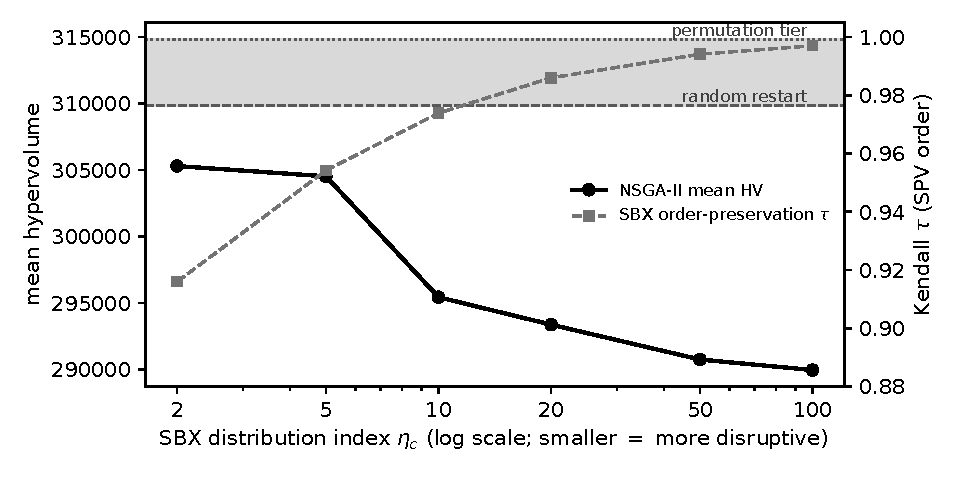
\includegraphics[width=0.66\textwidth]{eta_sweep.pdf}
\caption{Sweeping the SBX crossover distribution index $\eta_c$ for the real-coded NSGA-II on the visa problem. As $\eta_c$ falls (more disruptive crossover) the operator order-preservation $\tau$ drops, yet the mean hypervolume never reaches blind random restart (dashed), let alone the permutation tier (dotted); $\tau$ and \HV\ move in strictly opposite directions across the SBX sweep. SBX reaches at most $\tau=0.92$; the biased-uniform crossover ($\tau=0.63$) and HHO moves ($\tau\approx0$) extend the operator comparison in Section~\ref{sec:ablation}.}
\label{fig:eta}
\end{figure}

\begin{figure}[t]
\centering
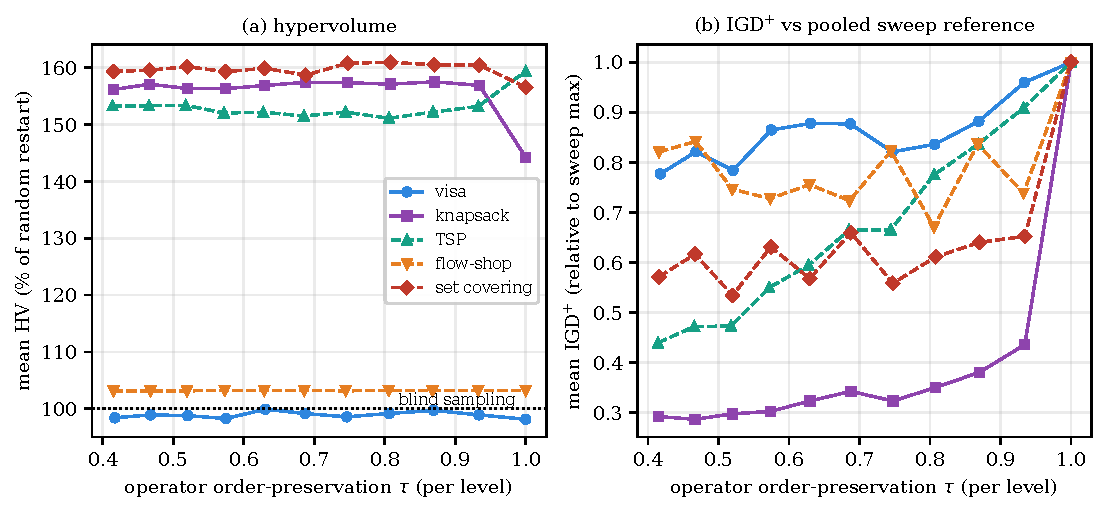
\includegraphics[width=\textwidth]{rho_sweep.pdf}
\caption{The registered dose--response sweep: the biased-uniform crossover's inheritance probability $\rho_e$ swept over eleven levels ($\tau\in[0.42,1.0]$, measured per level) under fixed NDS selection, on all five structures (30 seeds per level). (a)~Mean hypervolume as a percentage of each structure's blind random restart (dotted line): every curve is flat in $\tau$---the four-point sequence in the text is a family contrast, not a dose--response---with the visa below blind sampling throughout (by $0.1$--$1.9\,\%$) and the subset problems (knapsack, set covering) far above it. (b)~Mean IGD$^{+}$ against the pooled sweep front (relative to each structure's sweep maximum): coverage does degrade as $\tau\to1$ on the visa, knapsack, and TSP---a dose effect the $f_2$-dominated hypervolume does not register.}
\label{fig:rho}
\end{figure}

\paragraph{Operator and metaheuristic family are both second-order.}
The matched paradigms above all share the OX${}+{}$swap operators, so those comparisons varied the \emph{selection/replacement architecture} while holding the operator fixed. To probe the operator axis directly we ran a $3\times3$ factorial---three operator sets (OX${}+{}$swap, PMX (partially-mapped crossover)${}+{}$insertion, CX (cycle crossover)${}+{}$inversion) crossed with three of the architectures (permutation-NSGA-II, permutation-MOEA/D, and Discrete-MOHHO), 30 seeds each (Table~\ref{tab:factorial}). A two-way variance decomposition attributes just $5.5\,\%$ of the hypervolume variance to the operator set and $13.4\,\%$ to the architecture (interaction $2.9\,\%$), against $78.3\,\%$ from seed-to-seed noise; switching either axis moves the mean by at most ${\sim}2\,\%$ (operator marginal range $4{,}139$, architecture range $6{,}720$~\HV), an order of magnitude below the run-to-run variation. So \emph{once the representation is matched, neither the operator set nor the metaheuristic family governs performance}: the representation--operator match---the random-key$\to$permutation jump---is first-order, while both design axes within the matched representation are second-order. Discrete-MOHHO is the most operator-robust of all, holding ${\approx}317{,}000$~\HV\ across every operator set. Architecture is the larger of the two second-order effects ($13.4\,\%$ vs.\ $5.5\,\%$), and Discrete-MOHHO's energy-besiege architecture shows that a swarm can be made competitive once representation-matched; both effects remain an order of magnitude below the seed noise, so each is second-order relative to the first-order representation jump.

\begin{table}[t]
\centering
\caption{The method ladder: 30 runs each, identical greedy decoder and $25{,}000$-evaluation budget. Top block: random-key encoding (including the BRKGA-style predictive-test method and a competent MO-HHO that reaches the top tier); bottom block: permutation-native. A competent random-key method matches the permutation tier, so the encoding is not the performance divider---non-degenerate search is. Best per column in bold (rk-NSGA-II's combined front benefits from its high between-run dispersion---its bimodal runs explore different regions---while per-run it only ties blind sampling); ``perm-'' abbreviates ``permutation-''.}
\label{tab:ladder}
\small
\begin{tabular}{llccrr}
\toprule
\textbf{Method} & \textbf{Paradigm} & \textbf{Mean \HV\ $\pm\,\sigma$} & \textbf{CV} & \textbf{Comb.\ \HV} & \textbf{\#\,sols}\\
\midrule
NSGA-II            & GA       & $293{,}367 \pm 6{,}996$ & 2.38\,\% & 316{,}060 & 92\\
MOHHO              & swarm    & $302{,}756 \pm 7{,}138$ & 2.36\,\% & 320{,}984 & 104\\
rk-NSGA-II (biased unif.) & GA & $309{,}970 \pm 9{,}790$ & 3.16\,\% & \textbf{325{,}465} & 157\\
Random restart     & ---      & $310{,}214 \pm 2{,}735$ & 0.88\,\% & 317{,}673 & 65\\
Competent MO-HHO   & swarm    & $316{,}347 \pm 6{,}683$ & 2.11\,\% & 321{,}800 & \textbf{207}\\
\midrule
perm-MOEA/D                 & decomp.\ & $314{,}846 \pm 5{,}384$  & 1.71\,\% & 320{,}969 & 90\\
Discrete-MOHHO              & swarm    & $316{,}792 \pm 2{,}258$  & 0.71\,\% & 321{,}408 & 137\\
perm-SPEA2                  & str.-Pareto & $317{,}135 \pm 3{,}814$ & 1.20\,\% & 322{,}037 & 179\\
perm-NSGA-II                & GA       & $\mathbf{318{,}151 \pm 1{,}855}$ & \textbf{0.58\,\%} & 321{,}935 & 148\\
\bottomrule
\end{tabular}
\end{table}

\begin{table}[t]
\centering
\caption{Operator${}\times{}$architecture factorial on the visa problem: mean hypervolume (30 seeds) for three permutation operator sets crossed with three selection architectures, all under the matched budget. A two-way decomposition gives $\eta^2=5.5\,\%$ (operator), $13.4\,\%$ (architecture), $2.9\,\%$ (interaction), $78.3\,\%$ (seed noise): both design axes are second-order once the representation is matched.}
\label{tab:factorial}
\small
\begin{tabular}{lccc}
\toprule
\textbf{Operator set} & \textbf{perm-NSGA-II} & \textbf{perm-MOEA/D} & \textbf{Discrete-MOHHO}\\
\midrule
OX${}+{}$swap        & 317{,}237 & 313{,}608 & 317{,}569\\
PMX${}+{}$insertion  & 311{,}284 & 309{,}316 & 317{,}715\\
CX${}+{}$inversion   & 309{,}702 & 309{,}248 & 317{,}048\\
\bottomrule
\end{tabular}
\end{table}

\paragraph{An empirical regularity.}
The ladder (Figure~\ref{fig:ladder}) makes the pattern unmistakable: performance is governed by whether the search is \emph{non-degenerate}---operators that change the decoded order together with selection that preserves diversity---not by the encoding (random-key versus permutation) or the metaheuristic family. That encoding--operator mismatch can hurt search has been known since random keys were introduced~\cite{bean}, and the locality of decoder-based encodings was formalized by Rothlauf~\cite{rothlauf} and measured for single-objective decoder EAs by Raidl and Gottlieb~\cite{raidl}; our contribution is the controlled, multi-method, causally graded demonstration on a real constrained multi-objective problem---including the counterintuitive result that both real-coded searches (the standard NSGA-II and the MOHHO swarm) fall below blind sampling---and the decomposition of performance into decoder, representation, and family. That four distinct paradigms (swarm, decomposition, strength-Pareto, dominance/GA) converge to within about $1\,\%$ once the representation is matched, all far above the naive random-key methods, is strong evidence that the family is second-order here. We are precise about what this shows. The two conditions (an order-changing operator and diversity-preserving selection) are first-order: necessary, and graded in the operator's order disruption (the predictive test above); a competent random-key swarm satisfies both and joins the top tier, so the encoding itself is not the divider. Within a matched representation both the operator set and the selection/replacement architecture (Pareto sorting, scalarized decomposition, or energy-driven besiege) are second-order, the factorial of Table~\ref{tab:factorial} attributing only $5.5\,\%$ and $13.4\,\%$ of the variance to them. An omnibus test across all nine ladder methods on the common 30-seed block---a paired Friedman test with a Nemenyi post-hoc~\cite{demsar}, identical to the analysis of Section~\ref{sec:secondproblem}---rejects equal performance decisively ($\chi^2=133.8$, $p\approx4.6\times10^{-25}$, critical difference $2.19$). The mean ranks order the methods exactly as the two-condition account predicts: permutation-NSGA-II ($2.97$), competent MO-HHO ($3.10$), permutation-SPEA2 ($3.53$), Discrete-MOHHO ($3.93$), and permutation-MOEA/D ($4.33$) on top; the biased-uniform rk-NSGA-II ($4.57$) within the critical difference of random restart ($6.47$); the naive MOHHO ($7.33$) and the real-coded NSGA-II ($8.77$) at the bottom. Finer within-tier separations fall within the Nemenyi critical difference, consistent with the ``within about $1\,\%$'' clustering.

The ladder also survives leaving the hypervolume entirely: re-scoring every per-run front under IGD$^{+}$ and the additive $\epsilon$-indicator against a common reference front (the nondominated union of all $9\times30$ runs, $|Z_9|=187$) preserves the structure---rank correlations with the \HV\ ranking of $0.82$ and $0.85$, both omnibus tests decisive (Friedman $\chi^2=176.5$ and $169.3$)---with the four methods satisfying both conditions holding the top four ranks under all three indicators (permutation-SPEA2 is in fact best under both reference-free indicators) and the two degenerate real-coded methods at the bottom; the one displacement is permutation-MOEA/D, whose decomposition covers the pooled reference front poorly (rank $7.2$ under IGD$^{+}$) even though its per-run \HV\ stays in the tier. The headline pairwise claims are also multiplicity-robust: all twelve survive a Holm correction over the named family (largest surviving $p=5.7\times10^{-4}$). The ranking is also robust to the hypervolume reference point: across five reference points random restart outranks both real-coded searches throughout, and the strict permutation/random-key tier split holds under four of the five, breaking only at the tightest. We frame this as an empirical regularity for this problem, not a general law: all instances here share one structural skeleton---which the structurally distinct problems of Section~\ref{sec:secondproblem} directly address.

\begin{figure}[t]
\centering

\includegraphics[width=0.74\textwidth]{ladder.pdf}
\caption{The nine-method ladder: per-run hypervolume (30 runs each, identical decoder and budget). The divider is non-degenerate search, not the encoding: within the random-key block (left, shaded amber) the BRKGA-style rk-NSGA-II rises to---but only ties---blind random restart, while the competent MO-HHO joins the permutation-native top tier (right, shaded blue). Permutation-NSGA-II and Discrete-MOHHO are the tightest distributions (most stable).}
\label{fig:ladder}
\end{figure}

\paragraph{Robustness to a search-space-collapse confound.}
A skeptic could argue that the decoder's budget saturation collapses the search space so far that the optimizer is necessarily second-order. We tested this on three axes. \emph{Structure}: $50{,}000$ random permutations decode to $39{,}401$ distinct objective points (degeneration ratio $1.27$), and a principal-component analysis (PCA) places about $99\,\%$ of the front's variance in two components---the first component alone captures only $0.81$--$0.91$, so the effective problem is \emph{near-mono-objective}---one wide axis ($f_2$, $\sim$$39\times$ wider than $f_1$ across these random decodes) with a genuine but narrow second axis, a deliberately weak multi-objective lead case. \emph{Decoder}: re-running the full ladder on two \emph{non-saturating} decoders (a fractional-intensity and a stochastic-skip decoder, both feasible by construction) keeps the permutation tier significantly above the random-key tier under all three decoders (paired Wilcoxon $p<10^{-3}$) and never inverts it; the margin shrinks from $6.9\,\%$ (greedy) to $4.3\,\%$ (stochastic-skip) and $1.4\,\%$ (fractional-intensity), so saturation amplifies---it does not create---the effect, and an exact $(f_1,f_3)$ MILP front (with $f_2$ a posteriori---its visa-weighted mean waits are ratios of decision variables, outside MILP form) exposes no practically meaningful non-saturating solution the greedy front misses. \emph{Metric}: the GA operators' near-identity holds on the full decoded allocation, not just the order (an SBX step barely perturbs the decoded vector---consistent with its order near-identity $\tau=0.99$---whereas an HHO step moves it substantially), and the per-run tier ranking is reference-point-robust (above)---though on the combined fronts the strict tier softens under reference-free metrics (\IGD$^{+}$, additive $\epsilon$), which converge to a near-common reference set, so the tier is a per-run phenomenon, and the hypervolume that exhibits it is dominated by the $f_2$ axis---the only objective with a wide range, $f_1$ being more than an order of magnitude narrower and $f_3$ saturating. The confound thus bounds rather than overturns the claim: the effect is real and robust, modest on this saturation-amplified, $f_2$-dominated instance, with the general regularity resting on the additional structures below.

\subsection{Isolating the two conditions: a controlled $2\times2$}
\label{sec:twoconditions}
The ladder establishes the two conditions by observation; we now isolate each condition with a controlled $2\times2$ on a single real-coded random-key skeleton---same greedy decoder, instance, $25{,}000$-evaluation budget, and 30 seeds---varying only the \emph{operator} (order-changing HHO moves with mutation, $\tau\!\approx\!0$, versus near-identity SBX, $\tau\!=\!0.99$) and the \emph{selection} (diversity-preserving non-dominated sorting (NDS) versus dominance-gated acceptance). Table~\ref{tab:factorial2x2} shows that only the cell satisfying both conditions beats blind random restart ($315{,}730$ versus $310{,}214$~\HV, $+1.78\,\%$, Mann--Whitney $p=5.5\times10^{-5}$, $A_{12}=0.79$); either single-condition cell falls below blind sampling. Gated acceptance freezes the population (only $0.9\,\%$ of individuals move per iteration), and near-identity SBX leaves the decoded order almost unchanged even when the population does move. Crucially, the two conditions are synergistic, not additive: a two-factor analysis of variance finds a significant operator$\times$selection interaction ($\eta^2=0.098$, $F=16.7$, $p=8.0\times10^{-5}$), alongside main effects of $\eta^2=0.076$ (operator) and $\eta^2=0.145$ (selection). We read these effect sizes with the same yardstick as the factorial of Table~\ref{tab:factorial}: each is modest against seed noise, and the interaction matters not for its variance share but because it separates beating blind sampling from losing to it. Neither condition alone lifts performance above blind sampling---both single-condition cells lose by $1.4$--$2.0\,\%$---so the gain is genuinely a joint effect of changing the decoded order and preserving diversity. Figure~\ref{fig:mech2x2} maps each cell onto its operator $\tau$ and realized population movement, isolating the winning cell in the low-$\tau$, high-movement corner.

\begin{table}[t]
\centering
\caption{Controlled $2\times2$ isolating the two conditions on one real-coded random-key skeleton (visa decoder, 30 seeds, $25{,}000$ evaluations). Only the cell that both changes the decoded order and preserves diversity beats blind random restart ($310{,}214$~\HV); the operator$\times$selection interaction is significant. Best in bold.}
\label{tab:factorial2x2}
\small
\begin{tabular}{llrrr}
\toprule
\textbf{Operator} & \textbf{Selection} & \textbf{Mean \HV} & \textbf{vs.\ random} & \textbf{$A_{12}$}\\
\midrule
order-changing ($\tau\!\approx\!0$) & diversity (NDS) & $\mathbf{315{,}730}$ & $\mathbf{+1.78\,\%}$ & $\mathbf{0.79}$\\
order-changing ($\tau\!\approx\!0$) & gated            & $304{,}126$ & $-1.96\,\%$ & $0.24$\\
near-identity ($\tau\!=\!0.99$)     & diversity (NDS) & $305{,}892$ & $-1.39\,\%$ & $0.34$\\
near-identity ($\tau\!=\!0.99$)     & gated            & $304{,}760$ & $-1.76\,\%$ & $0.21$\\
\bottomrule
\end{tabular}
\end{table}
\begin{figure}[t]
\centering
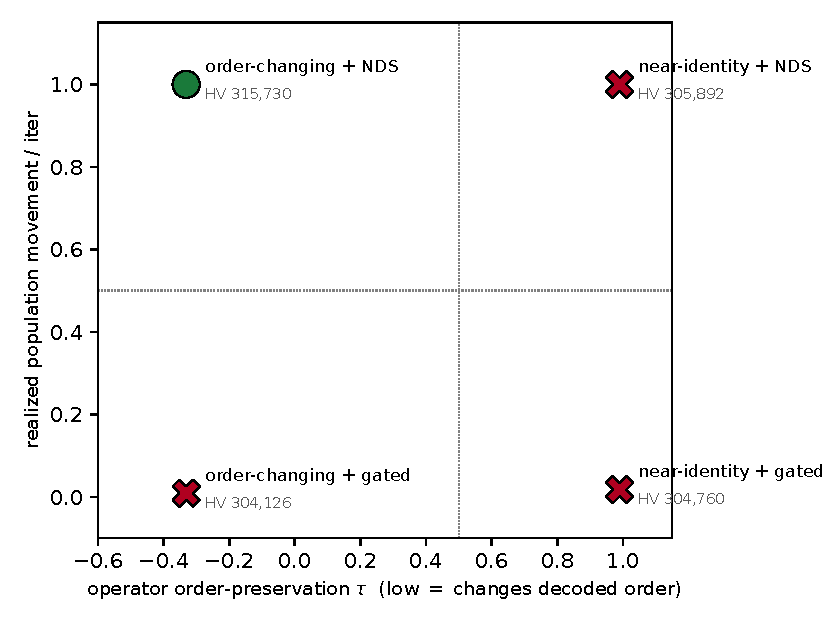
\includegraphics[width=0.68\textwidth]{mechanism_2x2.pdf}
\caption{Mechanism of the two conditions across the $2\times2$ cells: operator order-preservation $\tau$ (x) versus realized population movement per iteration (y), with each cell's mean \HV\ annotated. Only the order-changing, diversity-preserving cell occupies the favorable low-$\tau$, high-movement corner and beats blind sampling.}
\label{fig:mech2x2}
\end{figure}

\subsection{Generalization across instances}
\label{sec:generalization}

To check that these findings are not specific to a single backlog estimate, we built five further instances by perturbing every group's demand $n_g$ with an independent uniform $\pm 20\,\%$ jitter (fixed seeds) and recomputing the spillover-adjusted category caps and the per-country caps accordingly; on each we re-ran the full comparison (10 seeds per method). The pattern is invariant (Figure~\ref{fig:gen}): on all five perturbed instances---as on the base instance---the combined front dominates FIFO, MOHHO's mean hypervolume exceeds NSGA-II's (though with 10 seeds per instance the one-sided Mann--Whitney reaches only $p \le 0.071$ per instance: directionally consistent on five of five---two individually significant; since the five instances are perturbations of one instance rather than independent replicates, we read this as descriptive robustness, not confirmatory evidence), and the decoder-dominance signature persists, with random restart matching or exceeding MOHHO ($101$--$103\,\%$ of its hypervolume) and both above NSGA-II (which trails at $96$--$99\,\%$ of MOHHO). The pattern therefore holds across six instances, indicating that the conclusions are robust to $\pm 20\,\%$ demand-estimation error rather than artifacts of one estimate. We are careful not to overstate this: all six instances share the same structural skeleton (21 countries, 5 categories, the same caps and the demand-far-exceeds-supply regime), so this is robustness to demand perturbation; generalization across structurally distinct problems is addressed directly in Section~\ref{sec:secondproblem}.

\begin{figure}[t]
\centering
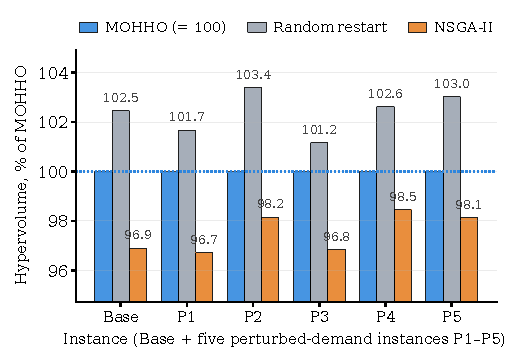
\includegraphics[width=0.74\textwidth]{generalization.pdf}
\caption{Generalization over six instances (base plus five $\pm 20\,\%$ perturbed-demand instances, P1--P5), each method's mean hypervolume shown as a percentage of MOHHO's on that instance. The ranking random restart $\ge$ MOHHO $>$ NSGA-II is preserved throughout ($101$--$103\,\%$ vs.\ $96$--$99\,\%$ of MOHHO); on every instance the combined front also dominates the FIFO baseline (not shown).}
\label{fig:gen}
\end{figure}

\subsection{Generalization across structurally distinct problems}
\label{sec:secondproblem}

The instances above share one structural skeleton. To test whether the regularity reaches genuinely different structures, we replicate the six-method core of the ladder on three further classic multi-objective combinatorial problems that share nothing with visa allocation but the SPV${}+{}$greedy/permutation methodology: a 0/1 \textbf{multidimensional knapsack} (MOMKP; 120 items, four capacities---a \emph{selection} landscape; its ladder is shown in Figure~\ref{fig:ladder2}), a tri-objective \textbf{traveling salesman} (mo-TSP; 100 cities, three cost matrices---a cyclic \emph{sequencing} landscape), and a tri-objective \textbf{permutation flow-shop} (mo-PFSP; 50 jobs, 10 machines; makespan, flowtime, and tardiness---a \emph{scheduling} landscape). Each runs the same six methods, budget, and 30 common seeds, analyzed by a paired Friedman test with a Nemenyi post-hoc (the Demšar standard~\cite{demsar}; Table~\ref{tab:structures}).

One result is robust across all four structures: among the six core ladder methods the best optimizer is always a permutation-native method (perm-NSGA-II on the visa, knapsack, and flow-shop problems; perm-MOEA/D on the TSP), and neither blind random restart nor any naive real-coded method is ever best (a competent real-coded swarm is a different story---see below). Matching the operators to the representation reliably produces the winner, and the metaheuristic family stays second-order among the matched methods. All four omnibus tests reject equality decisively (Friedman $\chi^2$ from $112$ to $150$, $p<10^{-21}$, critical difference $1.38$). We further placed the competent random-key MO-HHO of Section~\ref{sec:ablation} on all four structures (seven methods, same 30-seed budget): it wins outright on the knapsack (mean rank 1.13 of seven, above every permutation-native method) and ranks 2nd, 2nd, and 5th on the visa, flow-shop, and TSP, where a permutation-native method remains the single best. So the cross-structure regularity is sharper than ``permutation beats random-key'': what wins among the ladder methods on every structure is one satisfying both conditions---permutation-native on three of the four, the competent random-key swarm on the knapsack---and a competent random-key method joins the top tier rather than sitting in a separate encoding-defined tier. Our Discrete-MOHHO is a strong, low-variance matched optimizer that demonstrates the swarm-side mechanism, while permutation-NSGA-II is both the strongest and the steadiest matched method overall.

What does not generalize is the dramatic version of the story---a standard real-coded GA collapsing below blind random sampling. This holds on the two selection landscapes (visa and knapsack, where the real-coded NSGA-II is the worst method, beneath random restart) but reverses on the two sequencing landscapes: on the TSP and the flow-shop the real-coded NSGA-II is competitive (mean ranks $3.0$ and $2.7$) and random restart is instead the worst method. The mechanism reconciles this. Operator order-preservation is problem-independent---we re-confirmed $\tau$ on each problem's keys (SBX ${\approx}0.99$, HHO ${\approx}0$)---but its consequence is landscape-dependent: near-identity SBX leaves the decoded order almost frozen, which is fatal on selection landscapes (where blind sampling at least draws fresh subsets) yet acts as effective local search on sequencing landscapes (where small reorderings are precisely the useful neighborhood and blind sampling of full permutations is poor). Tuning sharpens the scoping further: granting the real-coded NSGA-II the same L9 on the knapsack lifts it $46\,\%$ above blind sampling ($0.290$ vs.\ $0.198$, $p=1.9\times10^{-9}$; winning row again $\eta_c{=}2$, $p_m{=}5/d$, i.e., mutation supplying the missing order disruption)---so the knapsack collapse is a default-configuration artifact, and the configuration-robust collapse is the visa's alone, where blind sampling sits within $2.6\,\%$ of the family-independent tier. We also asked whether a single ``search-headroom'' scalar predicts which structures show the collapse. A fifteen-point capacity sweep on the knapsack rules it out with power: the real-coded swarm captures a larger share of smaller gaps (Spearman $\rho=-0.78$, permutation two-sided $p=0.001$; descriptive, as the fifteen levels share one instance generator)---the scalar moves opposite to the hypothesis---so the exact landscape determinant remains open. The transferable claim is therefore narrow and precise: \emph{a method satisfying both conditions is the best optimizer on every structure (permutation-native on three of the four, the competent random-key swarm on the knapsack), and the metaheuristic family is second-order among them}; the spectacular ``GA-below-random'' collapse is a property of some selection/assignment landscapes---the registered set covering below, also subset-structured, does not show it---not a universal law. We report this scoping rather than the punchier over-generalization.

\paragraph{A registered prospective test.}
Every analysis above is retrospective in one respect: each problem was classified after its ladder had been run. As a final check we therefore registered the diagnostic's four predictions for a fifth, unseen problem before running any optimizer on it (the registration file and its git commit precede the results in the repository): a tri-objective \textbf{set-covering} problem (mo-SCP; 150 elements, 120 sets, three independent cost vectors; the SPV decoder adds a set iff it covers a still-uncovered element, so every decode is a full cover), which our registration---applying the protocol's step 3 as originally formulated---labeled a selection landscape by its subset structure. The two predictions that follow from the two conditions alone both held: permutation-NSGA-II and the competent random-key swarm beat blind sampling decisively (mean \HV\ $0.357$ and $0.386$ vs.\ $0.259$; one-sided $p=9.3\times10^{-10}$, $A_{12}=1.0$ for both). The two predictions tied to the landscape label both failed, informatively: the real-coded NSGA-II, predicted to collapse below blind sampling, instead finishes $10\,\%$ above it ($p=1.3\times10^{-8}$), and the biased-uniform rk-NSGA-II, predicted to tie blind sampling, is the single best method ($0.415$, $+60\,\%$ over blind sampling and significantly above permutation-NSGA-II, $p=9.3\times10^{-10}$). The reason is mechanistically clear in hindsight: mo-SCP has subset structure, but its decoder saturates no shared budget---every decode is feasible, and a marginal reordering swaps a single set of the cover---so the landscape behaves like a sequencing one (local search is useful, blind sampling weak) and an operator from the biased-uniform family wins---the family, not its disruption level, carrying the effect, consistent with the registered sweep of Section~\ref{sec:ablation}. The registered test thus confirms the two-condition core---order-renewal methods beat blind sampling on all five structures, and the best ladder method on every one of the five satisfies both conditions---while falsifying the surface structural label as a step-3 classifier (the protocol in Section~\ref{sec:discussion} therefore states step 3 as a baseline check). We note the asymmetry plainly: on a landscape where blind sampling proved weak, the two confirmed predictions carried less falsification risk than the two that failed---the test's value lies in the failures it localized. The sharpened, registration-backed open question is whether the operative determinant is the decoder's budget saturation leaving most random decodes near-equivalent---true on the visa and knapsack, false on mo-SCP---a hypothesis the headroom anti-correlation independently supports. A first operationalization---the budget-saturation share $s$, the mean utilization of the tightest decoder-enforced global resource over $1{,}000$ random decodes, computable in seconds---retrodicts where the default-configuration collapse occurred ($s=0.99$ on the visa, $1.00$ on the knapsack; $s=0$ by construction on TSP, flow-shop, and set covering, whose decoders cap no shared resource); the tuning control then narrows the configuration-robust regime to the visa, where blind sampling approaches the reachable frontier. We state this as retrodiction, not validation---all five outcomes were known---so registering the index's prediction on unseen problems is the natural follow-up.

\begin{table}[t]
\centering
\caption{Mean Friedman rank (lower is better; 30 common seeds, paired) of each method on four structurally distinct multi-objective problems. A permutation-native method is best on every structure among the six core methods (\textbf{bold}). At its default configuration the real-coded NSGA-II collapses below random restart only on the selection landscapes (visa, knapsack; tuning rescues the knapsack---see text); on the sequencing landscapes (TSP, flow-shop) it is competitive and random restart is the worst method instead. ``rk'' $=$ random-key encoding, ``pm'' $=$ permutation-native.}
\label{tab:structures}
\small
\begin{tabular}{llcccc}
\toprule
\textbf{Method} & \textbf{Enc.} & \textbf{Visa} & \textbf{Knapsack} & \textbf{TSP} & \textbf{Flow-shop}\\
\midrule
perm-NSGA-II        & pm & \textbf{1.60} & \textbf{1.10} & 2.00 & \textbf{1.80}\\
perm-MOEA/D         & pm & 2.53 & 2.87 & \textbf{1.00} & 2.83\\
Discrete-MOHHO      & pm & 2.23 & 2.10 & 4.00 & 2.63\\
\midrule
MOHHO (real-coded)  & rk & 4.67 & 3.93 & 5.00 & 5.07\\
Random restart      & rk & 4.20 & 5.23 & 6.00 & 5.93\\
NSGA-II (real-coded)& rk & 5.77 & 5.77 & 3.00 & 2.73\\
\bottomrule
\end{tabular}
\end{table}

\begin{figure}[t]
\centering
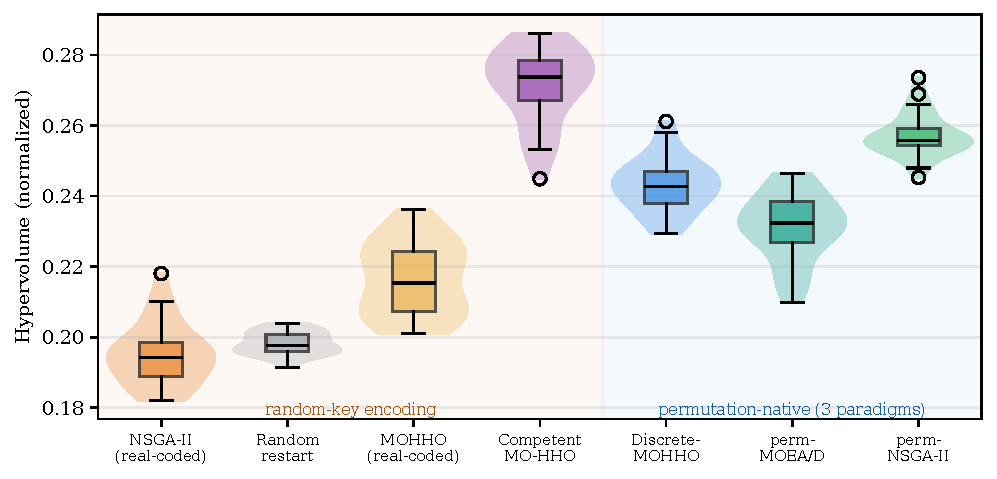
\includegraphics[width=0.78\textwidth]{ladder2.pdf}
\caption{The seven-method ladder on the multidimensional knapsack (MOMKP), one of the four structures of Table~\ref{tab:structures}. The naive random-key methods (NSGA-II and random restart) sit below the permutation-native methods, while the competent random-key swarm is the single best method here (mean rank 1.13 of seven)---so the divide is non-degenerate search, not the encoding. The split reverses on the sequencing landscapes (TSP, flow-shop), where the real-coded GA becomes competitive (Table~\ref{tab:structures}), and on the knapsack itself once the GA is tuned (see text).}
\label{fig:ladder2}
\end{figure}

%===============================================================================
\section{Discussion}
\label{sec:discussion}

\paragraph{The trade-off is structural.}
The conflict among objectives is not an artifact of the model. Two countries concentrate roughly three-quarters of demand with 10--13-year waits; the 7\,\% ceiling forbids fully serving them, so reducing disparity ($f_2$) forces unserved load to remain in those countries ($f_1\!\uparrow$), and distributing equitably leaves idle capacity in saturated categories ($f_3\!\uparrow$). The three extreme solutions of Table~\ref{tab:extremes} are mutually non-dominated---empirical proof of genuine three-way conflict.

\paragraph{Sensitivity.}
Two observations bound the result. First, the natural front holds only about 42 solutions per run---well under the size-100 archive cap, so pruning never activates and the archive size is immaterial (hypervolume unchanged from 100 to 500). Second, the range of $f_1$ across the front ($0.21$, vs.\ $f_2$'s ${\approx}11$~years) is more than an order of magnitude narrower: because total demand ($1{,}800{,}000$) far exceeds the $140{,}000$ visas, almost any permutation leaves a similar unserved load, so $f_1$ variability is constrained by the problem structure, not by the algorithm. We nonetheless keep $f_1$ as a distinct objective rather than collapsing to a two-objective $(f_2,f_3)$ problem: it still discriminates the efficiency-extreme solutions (Table~\ref{tab:extremes}) and makes the efficiency--equity tension explicit---indeed it is the minimum-$f_1$ policy that dominates FIFO, which a two-objective reduction would obscure.

\paragraph{A diagnostic protocol.}
The ladder distills into a protocol a practitioner can run before committing a full experimental budget to a decoder-based multi-objective method. \emph{Step 1 (operator check):} draw ${\sim}3{,}000$ parent--child pairs through the candidate operators and compute the Kendall $\tau$ between the parents' and children's decoded orders---minutes of computation, no full runs. \emph{Step 2 (selection check):} verify that selection preserves population diversity (non-dominated sorting, strength-Pareto, decomposition, or a crowded archive); dominance-gated acceptance fails this check (it froze all but $0.6\,\%$ of our population per iteration). \emph{Step 3 (baseline check):} measure how strong blind sampling is on the decoded space---run it; it is the cheapest method in any such comparison---rather than classifying the problem by surface structure: our registered prospective test (Section~\ref{sec:secondproblem}) shows the subset-versus-sequencing label can mispredict, the operative property appearing to be whether the decoder saturates a tight shared budget. The reliable, prospectively validated core is that the best ladder method on every one of the five structures satisfies both conditions, and order-renewal methods beat blind sampling on all five. On the budget-saturating problems (visa, knapsack), failing either check predicted default-configuration performance at or below blind sampling (the one nominal exception, the naive swarm on the knapsack, lies within the Nemenyi critical difference of random restart); on the visa, where blind sampling sits within $2.6\,\%$ of the best tier, no configuration of the random-key GA family beats it and only near-complete order renewal ($\tau\approx0$) cleared it; where blind sampling is weak relative to the reachable frontier (TSP, flow-shop, set covering---and, once tuned, the knapsack), other routes to order disruption suffice: local-search-like operators on sequencing problems, or simply a higher mutation rate (the knapsack's tuned GA). The registered sweep sharpens how to read step 1: $\tau$ is a flag, not a dial---within one operator family, eleven disruption levels move hypervolume by at most about one percentage point per $0.1\,\tau$ on all five structures (IGD$^{+}$ does degrade as $\tau\to1$ on three)---so treat the checks as qualitative; what transfers is that the measurements are cheap and the failure modes they flag are expensive. The protocol complements general fitness-landscape analysis~\cite{malan}: it measures the operator--decoder interaction rather than the landscape alone. Two further practical rules: invest design effort in the decoder and the representation before the search heuristic, and when a single dependable run matters---as in decision support---prefer a low-variance matched optimizer (permutation-NSGA-II strongest overall here, with Discrete-MOHHO the matched-swarm counterpart).

\paragraph{Policy implication.}
The front is a quantified map of compromises for a decision-maker, from prioritizing efficiency ($f_1=8.79$) to radical equity ($f_2=2.0$) or full utilization ($f_3=0$). Notably, reducing disparity from 13.0 to 2.0 years costs only about 2.4\,\% in $f_1$ relative to the FIFO baseline, indicating that large equity gains are attainable at modest efficiency cost---consistent with proposals to reform the per-country caps~\cite{crs,fwd}. A post-hoc audit over alternative country-wait fairness measures points in the same direction: relative to FIFO, front solutions reduce wait standard deviation from $3.14$ to $0.75$ years and Gini from $0.79$ to $0.17$, while increasing a Jain index on inverse waits from $0.80$ to $0.94$. Each front solution maps to a concrete allocation. Figure~\ref{fig:impact} shows the per-country reallocation of one balanced, full-utilization policy ($f_3=0$, $f_2=7.59$ years) against FIFO: it keeps the highest-demand countries (India, China, and the Philippines) at their 7\,\% ceiling and rebalances the rest---the residual ``Rest of World'' pool and several lower-served countries (Germany, Canada, Iran, and Nigeria) gain visas, drawn chiefly from the over-allocated Mexico and United Kingdom queues---an interpretable, auditable reallocation rather than an opaque score.

\begin{figure}[t]
\centering
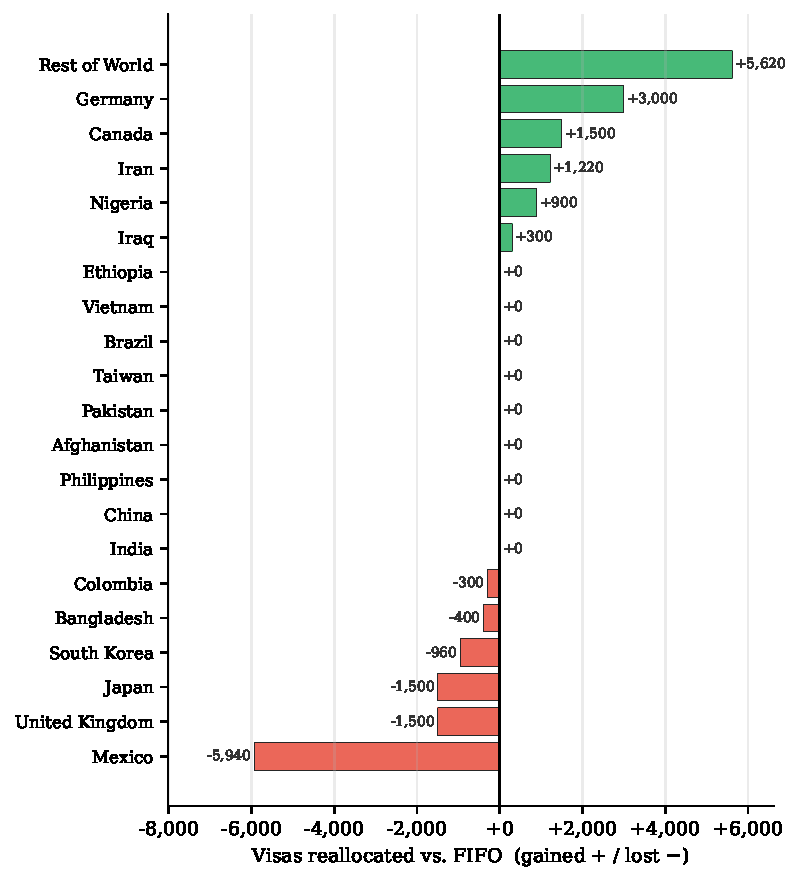
\includegraphics[width=0.72\textwidth]{country_impact.pdf}
\caption{Policy output: visas reallocated per country by a balanced full-utilization MOHHO solution relative to the FIFO baseline (gains as positive bars in blue, losses as negative bars in red). The highest-demand countries remain at their per-country ceiling; the gains accrue to the residual pool and several lower-served countries, drawn chiefly from over-allocated queues (notably Mexico).}
\label{fig:impact}
\end{figure}

\paragraph{Limitations.}
Four caveats bound the conclusions. The model covers a single fiscal year and ignores intertemporal backlog dynamics; it uses 21 representative countries rather than the full roster; demand $n_g$ is calibrated to published aggregate data~\cite{cato,uscis,dos} (although Section~\ref{sec:generalization} shows the comparison is stable under $\pm 20\,\%$ demand perturbations); and it assumes every assigned visa is used (no post-allocation refusals). These limitations affect external validity, not the internal comparison among the ladder methods, which all run on identical data with an identical decoder and budget.

%===============================================================================
\section{Conclusions}
\label{sec:conclusions}

We formulated a calibrated instance of the annual allocation of U.S.\ employment-based visas as a three-objective integer program with six hard constraints and searched the decoder-reachable trade-off space through a feasibility-preserving SPV${}+{}$greedy decoder that guarantees feasibility by construction---no penalties, no repair. A Taguchi L9 design fixed a common, confirmed operating point shared by every method. Across 30 independent runs the recovered Pareto front dominates the FIFO incumbent---chiefly by reducing waste while essentially matching its waiting load and maximal disparity---with 94 zero-waste solutions.

Our central result comes from a controlled nine-method ladder: blind random sampling beats a standard real-coded NSGA-II and the naive real-coded MOHHO swarm, but a competent real-coded swarm (HHO with non-dominated-sorting selection) beats blind sampling by $2.0\,\%$---so what fails is degenerate search, not real-coded search as such. The lesson is a two-condition diagnostic, scoped and graded. At default configuration on the budget-saturating problems---and under every configuration on the visa, where blind sampling approaches the reachable frontier---a method that does not change the decoded order or does not preserve population diversity falls to or below blind sampling (within the critical difference). In a predictive test, a method not used to formulate the rule---a BRKGA-style biased-uniform crossover that does change the order ($\tau=0.63$) under diversity-preserving selection---only ties blind sampling, so the two conditions are necessary but not sufficient. A second registered sweep (one operator, a continuous disruption knob, eleven levels, all five structures) finds hypervolume nearly flat in $\tau$ within the family (within about one percentage point per $0.1\,\tau$): the four-point gradient was a family contrast, not a dose--response, and only the right kind of order renewal ($\tau\approx0$ moves or permutation operators) reaches the visa top tier. There, four permutation-native paradigms (a GA, a strength-Pareto method, a decomposition method, and a Harris Hawks optimizer) cluster within about $1\,\%$ and a competent random-key swarm joins them---so the divider is non-degenerate search, not the encoding; Discrete-MOHHO improves on classic MOHHO by $4.6\,\%$ ($p=9.3\times10^{-10}$) and is the most stable swarm (CV $0.71\,\%$), within $0.5\,\%$ of the best (permutation-NSGA-II, the strongest and steadiest overall at CV $0.58\,\%$).

The FIFO-domination and decoder-dominance findings are directionally consistent across five perturbed-demand instances, and a four-structure study (knapsack, TSP, and flow-shop scheduling) sharpens what generalizes: the best ladder method on every structure satisfies both conditions (permutation-native on three, the competent random-key swarm on the knapsack) and the metaheuristic family is second-order among matched methods---the robust, transferable regularity---whereas the spectacular collapse of a mismatched real-coded GA below blind sampling occurs at default configuration on the budget-saturating landscapes (visa, knapsack) and is configuration-robust only on the visa---six controls (identical archive, canonical L\'evy, GRASP, per-family L9 tuning, Pareto local search, and a registered disruption sweep) show that nothing short of order renewal beats blind sampling there; on TSP and flow-shop the same near-identity operators act as useful local search and the GA is competitive. A registered prospective test on a fifth, unseen problem (a tri-objective set covering) confirms the core and sharpens the scope: order-renewal methods again beat blind sampling and the best ladder method again satisfies both conditions, but this subset-structured problem shows no GA collapse---the surface landscape label mispredicts, and the operative determinant (we hypothesize: decoder budget saturation) is the registered open question. A three-axis robustness analysis---non-saturating decoders, reference-point sweeps, and an exact MILP front---shows the representation effect is not created by the decoder's budget saturation but only amplified by it, modest on this $f_2$-dominated instance and carried, as a general regularity, by the replication structures. Operator order-preservation ($\tau{=}0.99$) is problem-independent; whether it freezes or refines is landscape-dependent, and the precise determinant we report as an open question (a fifteen-point sweep rules out a single search-headroom scalar, which moves opposite to the hypothesis: $\rho=-0.78$, $p=0.001$).

Beyond the numbers, the optimizer yields an auditable menu of feasible trade-off allocations: a decision-support artifact, not a policy prescription, given the single-period model and the representative (partly synthetic) instance. Future work includes a multi-period formulation, the full country roster, a legally detailed cross-preference spillover simulation, and testing the registered budget-saturation hypothesis as the landscape determinant.

%===============================================================================
\subsubsection*{Ethical Considerations.}
Allocating immigrant visas across nationalities is normatively charged. Our equity objective $f_2$ encodes one specific, contestable notion of fairness (minimizing the inter-country gap in mean wait), and the formulation treats nationalities as allocation buckets---a modeling choice with real human stakes, not a neutral given. We therefore frame the recovered front as decision support that makes trade-offs explicit and auditable, never as an autonomous decision-maker: any real-world use would require legal review, deliberation over which fairness criterion to adopt, and consultation with affected stakeholders. The instance is partly synthetic (see Section~\ref{sec:formulation}), so the per-country figures illustrate method behavior and must not be read as recommendations about real applicants.

%===============================================================================
\subsubsection*{Data and Code Availability.}
The problem data, the optimizer, the Taguchi design, and the scripts that reproduce every figure and table will be released in a public repository upon acceptance; an anonymized snapshot is available for review at \url{https://anonymous.4open.science/r/decoder-moo-reproducibility/}. The double-blind supplement includes a fast verifier that runs the unit tests, claim firewall, page-count check, and anonymous-ZIP scan. All randomized studies use fixed seeds---the diagnostic suite uses seed $1$, and the 30-run comparisons use a fixed seed block (seeds 1--30) recorded in the code---so the script regenerates every reported number deterministically.

%===============================================================================
\begin{thebibliography}{99}

\bibitem{alrafei}
Al Rafei, T., Yousfi Steiner, N., Chrenko, D.: Genetic algorithm and Taguchi method: an approach for better Li-ion cell model parameter identification. Batteries \textbf{9}(2), 72 (2023). \doi{10.3390/batteries9020072}

\bibitem{aranha}
Aranha, C., Camacho Villal\'on, C.L., Campelo, F., Dorigo, M., Ruiz, R., Sevaux, M., et al.: Metaphor-based metaheuristics, a call for action: the elephant in the room. Swarm Intelligence \textbf{16}(1), 1--6 (2022). \doi{10.1007/s11721-021-00202-9}

\bibitem{bansak}
Bansak, K., Ferwerda, J., Hainmueller, J., Dillon, A., Hangartner, D., Lawrence, D., et al.: Improving refugee integration through data-driven algorithmic assignment. Science \textbf{359}(6373), 325--329 (2018). \doi{10.1126/science.aao4408}

\bibitem{bean}
Bean, J.C.: Genetic algorithms and random keys for sequencing and optimization. ORSA Journal on Computing \textbf{6}(2), 154--160 (1994). \doi{10.1287/ijoc.6.2.154}

\bibitem{cato}
Bier, D.J.: 1.8 million in employment-based green card backlog. Cato Institute, Washington, DC (2023), \url{https://www.cato.org/blog/18-million-employment-based-green-card-backlog}

\bibitem{chaves}
Chaves, A.A., Resende, M.G.C., Schuetz, M.J.A., Brubaker, J.K., Katzgraber, H.G., de Arruda, E.F., et al.: A random-key optimizer for combinatorial optimization. Journal of Heuristics \textbf{31}(4), 32 (2025). \doi{10.1007/s10732-025-09568-z}

\bibitem{choo}
Choo, Y.H., Cai, Z., Le, V., Johnstone, M., Creighton, D., Lim, C.P.: Enhancing the Harris' Hawk optimiser for single- and multi-objective optimisation. Soft Computing \textbf{27}(22), 16675--16715 (2023). \doi{10.1007/s00500-023-08952-w}

\bibitem{coello}
Coello Coello, C.A., Lamont, G.B., Van Veldhuizen, D.A.: Evolutionary Algorithms for Solving Multi-Objective Problems, 2nd edn. Springer, New York (2007). \doi{10.1007/978-0-387-36797-2}

\bibitem{crs}
Congressional Research Service: U.S. employment-based immigration policy. Report R47164 (2023), \url{https://www.congress.gov/crs-product/R47164}

\bibitem{deb}
Deb, K., Pratap, A., Agarwal, S., Meyarivan, T.: A fast and elitist multiobjective genetic algorithm: NSGA-II. IEEE Transactions on Evolutionary Computation \textbf{6}(2), 182--197 (2002). \doi{10.1109/4235.996017}

\bibitem{demsar}
Demšar, J.: Statistical comparisons of classifiers over multiple data sets. Journal of Machine Learning Research \textbf{7}, 1--30 (2006), \url{https://jmlr.org/papers/v7/demsar06a.html}

\bibitem{derrac}
Derrac, J., García, S., Molina, D., Herrera, F.: A practical tutorial on the use of nonparametric statistical tests as a methodology for comparing evolutionary and swarm intelligence algorithms. Swarm and Evolutionary Computation \textbf{1}(1), 3--18 (2011). \doi{10.1016/j.swevo.2011.02.002}

\bibitem{feo}
Feo, T.A., Resende, M.G.C.: Greedy randomized adaptive search procedures. Journal of Global Optimization \textbf{6}(2), 109--133 (1995). \doi{10.1007/BF01096763}

\bibitem{fwd}
FWD.us: Per-country cap reform: priority bill spotlight (2024), \url{https://www.fwd.us/news/per-country-cap-reform-priority-bill-spotlight/}

\bibitem{garey}
Garey, M.R., Johnson, D.S.: Computers and Intractability: A Guide to the Theory of NP-Completeness. W.H. Freeman, San Francisco (1979)

\bibitem{gezici}
Gezici, H., Livatyali, H.: An improved Harris Hawks Optimization algorithm for continuous and discrete optimization problems. Engineering Applications of Artificial Intelligence \textbf{113}, 104952 (2022). \doi{10.1016/j.engappai.2022.104952}

\bibitem{goncalves}
Gon\c{c}alves, J.F., Resende, M.G.C.: Biased random-key genetic algorithms for combinatorial optimization. Journal of Heuristics \textbf{17}(5), 487--525 (2011). \doi{10.1007/s10732-010-9143-1}

\bibitem{heidari}
Heidari, A.A., Mirjalili, S., Faris, H., Aljarah, I., Mafarja, M., Chen, H.: Harris hawks optimization: algorithm and applications. Future Generation Computer Systems \textbf{97}, 849--872 (2019). \doi{10.1016/j.future.2019.02.028}

\bibitem{jangir}
Jangir, P., Heidari, A.A., Chen, H.: Elitist non-dominated sorting Harris hawks optimization: framework and developments for multi-objective problems. Expert Systems with Applications \textbf{186}, 115747 (2021). \doi{10.1016/j.eswa.2021.115747}

\bibitem{londe}
Londe, M.A., Pessoa, L.S., Andrade, C.E., Resende, M.G.C.: Biased random-key genetic algorithms: a review. European Journal of Operational Research \textbf{321}(1), 1--22 (2025). \doi{10.1016/j.ejor.2024.03.030}

\bibitem{malan}
Malan, K.M., Engelbrecht, A.P.: A survey of techniques for characterising fitness landscapes and some possible ways forward. Information Sciences \textbf{241}, 148--163 (2013). \doi{10.1016/j.ins.2013.04.015}

\bibitem{montgomery}
Montgomery, D.C.: Design and Analysis of Experiments, 9th edn. Wiley, Hoboken (2017)

\bibitem{rahimi}
Rahimi, I., Gandomi, A.H., Chen, F., Mezura-Montes, E.: A review on constraint handling techniques for population-based algorithms: from single-objective to multi-objective optimization. Archives of Computational Methods in Engineering \textbf{30}(3), 2181--2209 (2023). \doi{10.1007/s11831-022-09859-9}

\bibitem{raidl}
Raidl, G.R., Gottlieb, J.: Empirical analysis of locality, heritability and heuristic bias in evolutionary algorithms: a case study for the multidimensional knapsack problem. Evolutionary Computation \textbf{13}(4), 441--475 (2005). \doi{10.1162/106365605774666886}

\bibitem{rothlauf}
Rothlauf, F.: Representations for Genetic and Evolutionary Algorithms, 2nd edn. Springer, Berlin, Heidelberg (2006). \doi{10.1007/3-540-32444-5}

\bibitem{sorensen}
S\"orensen, K.: Metaheuristics---the metaphor exposed. International Transactions in Operational Research \textbf{22}(1), 3--18 (2015). \doi{10.1111/itor.12001}

\bibitem{tasgetiren}
Tasgetiren, M.F., Liang, Y.-C., Sevkli, M., Gencyilmaz, G.: A particle swarm optimization algorithm for makespan and total flowtime minimization in the permutation flowshop sequencing problem. European Journal of Operational Research \textbf{177}(3), 1930--1947 (2007). \doi{10.1016/j.ejor.2005.12.024}

\bibitem{uscis}
U.S. Citizenship and Immigration Services: Fiscal year 2023 employment-based adjustment of status FAQs (2023), \url{https://www.uscis.gov/green-card/green-card-processes-and-procedures/fiscal-year-2023-employment-based-adjustment-of-status-faqs}

\bibitem{dos}
U.S. Department of State: Visa bulletin for February 2026 (2026), \url{https://travel.state.gov/content/travel/en/legal/visa-law0/visa-bulletin/2026/visa-bulletin-for-february-2026.html}

\bibitem{vargha}
Vargha, A., Delaney, H.D.: A critique and improvement of the CL common language effect size statistics of McGraw and Wong. Journal of Educational and Behavioral Statistics \textbf{25}(2), 101--132 (2000). \doi{10.3102/10769986025002101}

\bibitem{cerci}
Wang, M., Wang, J.-S., Song, H.-M., Zhang, M., Zhang, X.-Y., Zheng, Y., et al.: Hybrid multi-objective Harris Hawk optimization algorithm based on elite non-dominated sorting and grid index mechanism. Advances in Engineering Software \textbf{172}, 103218 (2022). \doi{10.1016/j.advengsoft.2022.103218}

\bibitem{kusoglu}
Yüzgeç, U., Kuşoğlu, M.: Multi-objective Harris Hawks optimizer for multiobjective optimization problems. BSEU Journal of Engineering Research and Technology \textbf{1}(1), 31--41 (2020), \url{https://bseujert.bilecik.edu.tr/index.php/bseujert/article/view/14}

\bibitem{zhangli}
Zhang, Q., Li, H.: MOEA/D: a multiobjective evolutionary algorithm based on decomposition. IEEE Transactions on Evolutionary Computation \textbf{11}(6), 712--731 (2007). \doi{10.1109/TEVC.2007.892759}

\bibitem{zhang}
Zhang, W., Xiao, G., Gen, M., Geng, H., Wang, X., Deng, M., et al.: Enhancing multi-objective evolutionary algorithms with machine learning for scheduling problems: recent advances and survey. Frontiers in Industrial Engineering \textbf{2}, 1337174 (2024). \doi{10.3389/fieng.2024.1337174}

\bibitem{spea2}
Zitzler, E., Laumanns, M., Thiele, L.: SPEA2: improving the strength Pareto evolutionary algorithm. TIK-Report 103, Computer Engineering and Networks Laboratory (TIK), ETH Zurich (2001). \doi{10.3929/ethz-a-004284029}

\bibitem{zitzler}
Zitzler, E., Thiele, L.: Multiobjective evolutionary algorithms: a comparative case study and the strength Pareto approach. IEEE Transactions on Evolutionary Computation \textbf{3}(4), 257--271 (1999). \doi{10.1109/4235.797969}

\end{thebibliography}

\end{document}
